\chapter{若当标准形}

本讲我们将在前面讨论的基础上实现复数域上相似标准形理论的终极目标，即得到复数域上全体线性变换都可以得到的一种比较简单的矩阵表示——若当标准形. 我们将讨论其存在与唯一性，并在证明唯一性的过程中给出一种求解若当标准形的方法. 最后，我们将讨论若当标准形的应用.

\section{若当标准形的存在性}
回顾\autoref{thm:不变子空间与分块对角矩阵}，我们知道寻找线性变换$T\in\mathcal{L}(V)$在基下简单的表示矩阵的一般思路是将$V$分解为一系列不变子空间的直和. 在对角化一节中我们尝试分解为一维不变子空间的直和，但这并不能对所有的线性变换都成立，于是我们进一步在\autoref{thm:广义特征性质} 中对于任意的线性变换都利用广义特征子空间实现了这一分解，这也直接导出了\autoref{thm:分块对角矩阵} 中的分块对角形矩阵表示. 然而我们仍无法满足于将这一矩阵表示作为标准形，因为我们还希望分块对角矩阵中每个分块都要足够简单，即有一定的规律且有较多的零元素，所以我们需要对广义特征子空间做进一步的分解，并且取特定形式的基来实现这一目标. 我们首先看如下例子：

\begin{example}{}{}
    设$\sigma\in\mathcal{L}(\mathbf{C})^6$满足
    \[\sigma(x_1,x_2,x_3,x_4,x_5,x_6)=(2x_1+x_2,2x_2+x_3,2x_3,2x_4,3x_5+x_6,3x_6),\]
    则我们很容易写出其在$\mathbf{C}^6$自然基下的矩阵表示为
    \[\left(\begin{array}{ccc:c:cc}
                2 & 1 & 0 & 0 & 0 & 0 \\
                0 & 2 & 1 & 0 & 0 & 0 \\
                0 & 0 & 2 & 0 & 0 & 0 \\
                \hdashline
                0 & 0 & 0 & 2 & 0 & 0 \\
                \hdashline
                0 & 0 & 0 & 0 & 3 & 1 \\
                0 & 0 & 0 & 0 & 0 & 3 \\
            \end{array}\right)\]
\end{example}

通过这一例子我们观察到线性变换的一种分块对角矩阵表示，其中每个分块都十分简单，很适合作为我们实现为复数域上任意线性变换寻找的标准形. 我们称如上例矩阵表示的每个分块的形式的矩阵为\term{若当块}\index{ruodangkuai@若当块 (Jordan block)}，更严谨地，域$\mathbf{F}$上的一个$r$级矩阵形如\[\begin{pmatrix}
        \lambda & 1       &        &         \\
                & \lambda & \ddots &         \\
                &         & \ddots & 1       \\
                &         &        & \lambda
    \end{pmatrix}\]
则称其为一个$r$级若当块（1级显然就是1阶矩阵），记作$J_r(\lambda)$，其中$\lambda$是对角线上元素. 若一个线性变换$\sigma$在基$B$下的矩阵表示是对角块均为若当块的分块对角矩阵，则称这个分块对角矩阵是线性变换$\sigma$的\term{若当标准形}\index{ruodangxing@若当标准形 (Jordan canonical form)}，而这组基$B$称为$T$的\term{若当基}\index{ruodangji@若当基 (Jordan basis)}. 我们希望复数域上任意线性变换都能找到一组若当基使其矩阵表示为若当标准形，而这正是本节需要证明的目标.

为了证明这一结果，我们需要首先观察若当块能在怎样的基下表示出. 为了发现这一规律，我们考虑一种最简单的情况，即一个线性变换$T$在某组基$B=\{v_1,v_2,v_3,\ldots,v_n\}$下的矩阵表示就是一个若当块，即
\[\sigma(v_1,v_2,v_3,\ldots,v_n)=(v_1,v_2,v_3,\ldots,v_n)\begin{pmatrix}
        \lambda & 1       &        &         \\
                & \lambda & \ddots &         \\
                &         & \ddots & 1       \\
                &         &        & \lambda
    \end{pmatrix},\]
所以我们根据线性映射矩阵表示的定义可以得到
\begin{align*}
    \sigma(v_1) & =\lambda v_1,         \\
    \sigma(v_2) & =\lambda v_2+v_1,     \\
    \sigma(v_3) & =\lambda v_3+v_2,     \\
                & \cdots                \\
    \sigma(v_n) & =\lambda v_n+v_{n-1}.
\end{align*}

我们稍作变换，可以得到
\begin{equation} \label{eq:17:若当基的推导}
    \begin{aligned}
        (\sigma-\lambda I)v_1 & =0,       \\
        (\sigma-\lambda I)v_2 & =v_1,     \\
        (\sigma-\lambda I)v_3 & =v_2,     \\
                              & \cdots    \\
        (\sigma-\lambda I)v_n & =v_{n-1}.
    \end{aligned}
\end{equation}

即我们需要的这组基实际上具有如下形式：
\[B=\{(\sigma-\lambda I)^{n-1}(v_n),(\sigma-\lambda I)^{n-2}(v_n),\ldots,(\sigma-\lambda I)(v_n),v_n\},\]
并且有$(\sigma-\lambda I)^n=0$. 事实上观察上面这组等式，从第一个式子我们知道$v_1$实际上是$\sigma$关于特征值$\lambda$的特征向量，$v_2,\ldots,v_n$则是关于特征值$\lambda$的广义特征向量.

再进一步观察这样的一组向量，我们发现这组向量似乎与\autoref{thm:循环子空间} 中提到的循环基有些类似：它们都是从一个向量开始，不断作用一个线性变换等到的一组向量. 这里我们给出一个定义来详细地说明一些术语：
\begin{definition}{}{若当循环基}
    设$\sigma\in\mathcal{L}(V)$，$v\in V$是关于特征值$\lambda\in\mathbf{C}$的一个广义特征向量. 设$n$是使得$(\sigma-\lambda I)^n v=0$成立的最小正整数，则称$\{(\sigma-\lambda I)^{n-1}(v),(\sigma-\lambda I)^{n-2}(v),\ldots,(\sigma-\lambda I)(v),v\}$是 \term{$\sigma$关于特征值$\lambda$的循环广义特征向量组}（不引起歧义的情况下也可称循环向量），其中$(\sigma-\lambda I)^{n-1}(v)$称为其起始向量，$v$称为其终止向量.
\end{definition}

给出这一定义后，便可以开始研究这一组向量与我们目标中的若当基之间的关联. 我们需要暂时停下前进的脚步，仔细思考我们需要什么. 我们的最终目标是证明，对于任意复向量空间上的线性变换，都能找到一组基，其矩阵表示为分块对角矩阵，且每一对角块为若当块. 根据\autoref{thm:不变子空间与分块对角矩阵}，我们要求每个若当块对应的基向量张成的子空间是不变子空间，因为这样才能保证生成一个对角块. 而根据之前的推导，我们知道生成若当块必须要这样的一组循环向量，那么自然地会有两个问题：
\begin{enumerate}
    \item 循环向量生成的子空间一定是不变子空间吗？因为这样才能保证生成一个对角块；
    \item 我们是从一组基$v_1,\ldots,v_n$可以得到若当块出发定义出这样的循环向量的，那么是不是一组向量满足这样的定义也一定线性无关的呢？因为这样只需要找到这样一组循环向量就一定可以构成若当基的一部分.
\end{enumerate}
事实上如果读者熟悉之前讨论的一些例子和性质，这两个问题可以轻松解决：
\begin{theorem}{}{若当循环基的性质}
    设$\sigma\in\mathcal{L}(V)$，$B$是$\sigma$关于特征值$\lambda$的循环广义特征向量组，则
    \begin{enumerate}
        \item $B$是线性无关的，因此可以构成$\spa(B)$的一组基，称其为一组\term{若当循环基}；
        \item $B$生成的子空间$W$是$\sigma$的不变子空间（就是\autoref{def:循环子空间} 定义的循环子空间）.
    \end{enumerate}
\end{theorem}
\begin{proof}
    \begin{enumerate}
        \item 由$B$的生成过程\autoref{eq:17:若当基的推导} 和\autoref{ex:特征向量生成线性无关组}，线性无关性是显然的推论.
        \item 由$B$的定义（注意$(\sigma-\lambda I)^n v=0$）以及\autoref{thm:循环子空间}，$W$是$\sigma$的不变子空间.
    \end{enumerate}
\end{proof}

在以上问题被解决后，我们的目标将非常清晰，即对任意的复数域上的线性变换是否一定能找到一组基是由不同的若当循环基合并而成的，从而在在这组基下的矩阵表示是若当标准形？似乎有些困难，我们需要一些观察：事实上，若当循环基中的每个向量都是关于某个特征值$\lambda$的广义特征向量，因此它们张成的子空间应当是广义特征子空间$G_\lambda$的一部分（当然也可能张成整个广义特征子空间）. 于是站在\autoref{thm:广义特征性质} 中广义特征子空间分解的基础上，我们的目标可以转化为对其中的每一个广义特征子空间，找到一组由一个或多个若当循环基合并而成的基. 这样首先利用\autoref{thm:广义特征性质} 中广义特征子空间分解，再利用广义特征子空间的若当循环基分解，我们就可以得到一组由不同的若当循环基合并而成的基，从而得到若当标准形.

为了更清晰地展示，我们将上述过程形式化. 设$\sigma\in\mathcal{L}(V)$，$\lambda_1,\ldots,\lambda_m$是$\sigma$的互异特征值，$G_{\lambda_i}$是关于特征值$\lambda_i$的广义特征子空间. 根据\autoref{thm:广义特征性质}，我们知道
\[V=G_{\lambda_1}\oplus\cdots\oplus G_{\lambda_m}=\bigoplus_{i=1}^m G_{\lambda_i},\]
然后我们希望为每个广义特征子空间选取一组由一个或多个若当循环基合并而成的基，也就是说我们希望将每个广义特征子空间分解为一个或多个循环子空间的直和. 形式化而言，我们希望每个广义特征子空间$G_{\lambda_i}$可以由$s_i$组若当循环基$B_{i1},B_{i2},\ldots,B_{is_i}$张成，其中每一组基都可以表达为：
\[B_{ij}=\{(\sigma-\lambda_iI)^{r_{ij}-1}(v_{ij}),(\sigma-\lambda_iI)^{r_{ij}-2}(v_{ij}),\ldots,v_{ij}\},\]
事实上$r_{ij}$就是这组若当循环基的长度. 我们设由$B_{ij}$张成的循环子空间为$C_{ij}$，则有
\[G_{\lambda_i}=C_{i1}\oplus C_{i2}\oplus\cdots\oplus C_{is_i}=\bigoplus_{j=1}^{s_i} C_{ij},\]
再结合\autoref{thm:广义特征性质} 的分解，我们有
\begin{equation} \label{eq:17:循环子空间分解}
    V=\bigoplus_{i=1}^m G_{\lambda_i}=\bigoplus_{i=1}^m\bigoplus_{j=1}^{s_i} C_{ij}.
\end{equation}

根据\autoref{thm:若当循环基的性质}，每个循环子空间都是不变子空间，并且每个若当循环基都对应于一个若当块. 回忆我们上面的推导过程，我们现在剩下的任务就是为复数域上的任意广义特征子空间$G_{\lambda_i}$找到一组由一个或多个若当循环基合并而成的基，这样就能得到\autoref{eq:17:循环子空间分解} 所示的分解，从而得到任意复数域上的线性变换都存在若当标准形. 为了实现这一目标，我们需要先证明一个关于若当循环基的性质.

\begin{lemma}{}{若当循环基合并性质}
    设$\sigma\in\mathcal{L}(V)$，$\lambda\in\mathbf{C}$是$\sigma$的一个特征值. 设$B_1,\ldots,B_q$都是$\sigma$关于特征值$\lambda$的一组若当循环基，且它们的起始向量各不相同且构成了一组线性无关向量组，则
    \begin{enumerate}
        \item $B_i(i=1,\ldots,q)$是互不相交的；
        \item $B=B_1\cup\cdots\cup B_q$是线性无关向量组.
    \end{enumerate}
\end{lemma}
\begin{proof}
    \begin{enumerate}
        \item 反证法. 假设$B_i$和$B_j$有交集，即存在$v\in B_i\cap B_j$. 设$B_i$和$B_j$的终止向量分别为$v_i$和$v_j$，则存在非负整数$m_i,m_j$使得
              \[(\sigma-\lambda I)^{m_i}(v_i)=(\sigma-\lambda I)^{m_j}(v_j)=v.\]
              故$(\sigma-\lambda I)^{m_i+m}(v_i)=(\sigma-\lambda I)^{m_j+m}(v_j)$，其中$m$是任意非负整数，因此$B_i$和$B_j$从向量$v$开始一直到起始向量必定都是相等的，而这与定理的前提起始向量各不相同矛盾，故$B_i(i=1,\ldots,q)$是互不相交的.

        \item 同样反证法，假设$B$是线性相关向量组，则一定存在一个子向量组$u_1,\ldots,u_s$，使得有全部非零的$k_1,\ldots,k_s$使得
              \begin{equation} \label{eq:17:若当循环基合并性质证明}
                  k_1u_1+\cdots+k_su_s=0.
              \end{equation}
              这是一定能做到的，因为$B$线性相关表明存在一个向量$u_1$能被其它向量线性表示，我们写出这一线性表示，去除表示中系数为0的向量，又$u_1\neq 0$，故一定剩余一组向量满足
              \[u_1=c_2u_2+\cdots+c_su_s,\]
              其中$c_i\neq 0$，则$-u_1+c_2u_2+\cdots+c_su_s=0$，这就满足\autoref{eq:17:若当循环基合并性质证明} 中$k_1,\ldots,k_s$全部非零.

              接下来我们可以对每个$u_i$作用$(\sigma-\lambda I)$的幂次，在经过某个幂次后，所有的$u_i$都会变成它所在的$B_j$的起始向量. 假设每个$u_i$在作用$(\sigma-\lambda I)^{r_i}$次后变成所在$B_j$的起始向量，我们取$r=\max\{r_1,\ldots,r_s\}$，然后在\autoref{eq:17:若当循环基合并性质证明} 两边作用$(\sigma-\lambda I)^r$，则可以得到
              \begin{equation}
                  k_{i_1}(\sigma-\lambda I)^r(u_{i_1})+\cdots+k_{i_t}(\sigma-\lambda I)^r(u_{i_t})=0,
              \end{equation}
              其中$u_{i_1},\ldots,u_{i_t}$是$u_1,\ldots,u_s$中在作用$(\sigma-\lambda I)^r$后变成对应起始向量的向量，即$(\sigma-\lambda I)^r(u_{i_j})$都是起始向量，而其它向量已经到达超出起始向量所需次数，因此被化零. 又$k_{ij}$全都不为0，因此这些起始向量$(\sigma-\lambda I)^r(u_{i_j})$线性相关，这与定理的前提起始向量线性无关矛盾，故$B$是线性无关向量组.
    \end{enumerate}
\end{proof}

接下来我们便可以证明本节最核心的一个结果，即复数域上任意一个广义特征子空间都有一组由互不相交的循环基并起来构成的基，从而我们可以进一步利用广义特征子空间分解得到每个线性变换都有一组基使得其矩阵表示为若当标准形：
\begin{theorem}{}{广义特征子空间分解若当基}
    设$V$是$\mathbf{C}$上的有限维线性空间，$\sigma\in\mathcal{L}(V)$，$G_\lambda$是关于特征值$\lambda$的广义特征子空间，则$G_\lambda$有一组由不相交的若当循环基取并集构成的基.
\end{theorem}
\begin{proof}
    我们对$G_\lambda$的维数进行归纳. 维数等于1时结论显然成立. 我们假设对于维数小于$n$的情况结论成立，现在考虑$G_\lambda$维数为$n$的情况，由于使用归纳法，我们需要构造出一个维数更低的广义特征子空间. 我们考虑限制线性变换$(\sigma-\lambda I)\vert_{G_\lambda}$，我们知道这一定不是单射，因为$\lambda$是$\sigma$的特征值，因此$(\sigma-\lambda I)v=0$在$G_\lambda$内一定有非零向量解（实际上就是特征向量），因此由\autoref{thm:双射等价条件}，这也不是满射，因此$\dim\im(\sigma-\lambda I)\vert_{G_\lambda}<\dim G_\lambda$.

    我们记$U=\im(\sigma-\lambda I)\vert_{G_\lambda}$，这是一个维数更低的子空间，现在我们需要说明它是某个线性变换的广义特征子空间. 事实上我们可以直接考虑$\sigma\vert_U$，因为$\sigma$在全空间$V$上关于特征值$\lambda$的广义特征子空间是$G_\lambda$，因此限制在$G_\lambda$的子集上的映射$\sigma\vert_U$关于特征值$\lambda$的广义特征子空间必然就是$U$，因为对于任意的$u\in U\subset G_\lambda$，必然存在正整数$j$使得$(\sigma-\lambda I)^ju=0$. 于是根据归纳假设，$U$有一组由不相交的若当循环基取并集构成的基，记作$B=B_1\cup B_2\cup\cdots\cup B_q$（因为是基所以起始向量也必定线性无关）.

    于是接下来我们要将这组基扩充成$G_\lambda$的一组基，并保持若当循环基的特点. 观察$U=\im(\sigma-\lambda I)\vert_{G_\lambda}$和$G_\lambda$的区别，其一在于$\sigma-\lambda I$将$G_\lambda$的一些向量映射进了$U$，但这些向量本身不在$U$中，其二在于$\sigma-\lambda I$将$G_\lambda$中的一些向量（实际上就是特征向量）化零，而这些特征向量不在$U$中，因此我们就从这两个角度扩充.
    \begin{enumerate}
        \item 我们考虑任一若当循环基$B_i$的终止向量，它应当是某个$v_i\in G_\lambda$在$\sigma-\lambda I$下的像，我们直接将$v_i$加入到$B_i$中，这样我们就得到了$\tilde{B_i}=B_i\cup\{v_i\},\enspace i=1,\ldots,q$，它们仍然是满足循环向量组定义的.
        \item $B$中的特征向量实际上就是每个$B_i$的起始向量，我们记为$w_1,\ldots,w_q$，它们是特征子空间$V_\lambda$的一组线性无关向量，因此可以将其扩充为$V_\lambda$的一组基
              \[w_1,\ldots,w_q,u_1,\ldots,u_s.\]
    \end{enumerate}

    从而扩张后我们得到新的一组不相交且起始向量线性无关的若当循环基的并：
    \[\tilde{B}=\tilde{B_1}\cup\tilde{B_2}\cup\cdots\cup\tilde{B_q}\cup\{u_1\}\cup\cdots\cup\{u_s\},\]

    由\autoref{lem:若当循环基合并性质}，$\tilde{B}$必然线性无关. 最后我们证明$\tilde{B}$是$G_\lambda$的一组基. 假设$B$包含$r=\dim U$个向量，于是$\tilde{B}$包含$r+q+s$个向量. 又因为$w_1,\ldots,w_q,u_1,\ldots,u_s$是$V_\lambda$的一组基，而$V_\lambda=\ker(\sigma-\lambda I)\vert_{G_\lambda}$，由线性映射基本定理，
    \[\dim G_\lambda=\dim\ker(\sigma-\lambda I)\vert_{G_\lambda}+\dim\im(\sigma-\lambda I)\vert_{G_\lambda}=q+s+r,\]

    因此$\tilde{B}$线性无关且长度等于$G_\lambda$的维数，故是$G_\lambda$的一组若当循环基. 这样我们就完成了归纳过渡的证明，由归纳法知结论成立.
\end{proof}

由此，我们证明了复数域上线性变换的广义特征子空间一定有一组由若干个若当循环基合并而成的基，根据\autoref{eq:17:循环子空间分解} 的推导过程，下面这一定理也就自然成立：
\begin{corollary}{}{若当基存在}
    设$V$是$\mathbf{C}$上的有限维线性空间，$\sigma\in\mathcal{L}(V)$，则存在一组基$B$使得$\sigma$在$B$下的矩阵表示为若当标准形.
\end{corollary}

接下来我们需要描述矩阵的若当标准形. 实际上，线性变换在某组基下有若当标准形与矩阵有相似标准形为若当标准形是等价的，这一点与之前对角化、分块对角化等是一致的，因此我们很容易得到如下推论：
\begin{corollary}{}{}
    对复数域上的任意$n$阶矩阵$A$，都存在一个$n$阶矩阵$P$，使得$P^{-1}AP$是若当标准形.
\end{corollary}

至此我们已经证明对于复数域上的任意线性变换和矩阵，若当标准形的存在性，接下来我们将讨论若当标准形的唯一性，并在这一过程中讨论如何求解若当标准形和对应的基或者过渡矩阵.

\section{若当标准形的唯一性}

在上一节内容中，我们已经证明对于复数域上的任意线性变换和矩阵，都能有一组基或者过渡矩阵得到若当标准形. 本节我们将回答一个重要的问题，即一个线性变换或矩阵是否可能有两种若当基或过渡矩阵的取法，得到不同的若当标准形？我们的答案是否定的，并且在回答问题的过程中我们将给出获得这一唯一若当标准形的方法.

回忆\autoref{eq:17:循环子空间分解}，我们的目标应当是为每一个广义特征子空间找到一组由若当循环基合并而成的基，然后将这些基合并成一组基，从而得到若当标准形. 因此我们只需要讨论如何对某一个特征值$\lambda$对应的广义特征子空间$G_\lambda$找到一组由一个或多个若当循环基合并而成的基即可，当一个线性变换或矩阵有多个特征值时，只需要对每一个特征值对应的广义特征子空间做同样的操作即可.

因此我们现在只考虑将映射限制于一个广义特征子空间$G_\lambda$上的情形，将该特征值对应的若当块和若当基求解出来即可. 考虑到若当基是由一系列若当循环基合并而成，而若当循环基中会出现大量的$\sigma-\lambda I$的幂次. 回忆\autoref{thm:广义特征性质}，我们知道$(\sigma-\lambda I)\vert_{G_\lambda}$是幂零线性变换，因此我们可以自然地简记$N=\sigma-\lambda I$. 假设最终我们求得限制在$G_\lambda$下的若当基中有$n$组若当循环基，每组若当循环基的长度分别为$m_1,\ldots,m_n$（不妨设$m_1\geqslant\cdots\geqslant m_n$），则我们可以将这些若当基记为：
\[N^{m_1}v_1,\ldots,Nv_1,v_1,\ldots,N^{m_n}v_n,\ldots,Nv_n,v_n.\]

事实上这里有两组未知量，其一是每组若当循环基的长度$m_i$，这对应每个若当块的大小，因为每组若当循环基就对应于一个若当块；其二是每组若当循环基的终止向量$v_i$，这就可以决定出整个若当基. 我们接下来将分成两步来求解这两组未知量，我们将用到一个重要的工具，我们称其为\term{Young图}，如\autoref{fig:17:若当基Young图形式}. 这是一种倒三角形的方格图，每一列都是一组若当循环基，按照长度从长到短依次从左到右排列，这是从列的角度看Young图.

在利用Young图求解的过程中，我们也需要从行的角度来看Young图，这时需要引入一个新的记号方便我们的求解：我们记$G_j(\lambda,\sigma)=\ker N^j$（其中$N=\sigma-\lambda I$）. 根据\autoref{thm:核空间性质} 中的核空间增长性质，我们知道当$i<j$时有$G_i(\lambda,\sigma)\subseteq G_j(\lambda,\sigma)$. 最后，在求解之前，我们需要一个引理表明下述方法的合理性：
\begin{lemma}{}{Young图行性质}
    设$\sigma\in \mathcal{L}(V)$，若$V$中向量$v\in G_j(\lambda,\sigma)\backslash G_{j-1}(\lambda,\sigma)$，记$N=\sigma-\lambda I$，则对任意的$i<j$，有$N^iv\in G_{j-i}(\lambda,\sigma)\backslash G_{j-i-1}(\lambda,\sigma)$.
\end{lemma}

\begin{proof}
    % \begin{enumerate}
    %     \item 直接利用定义，$v\in G_j(\lambda,\sigma)\backslash G_{j-1}(\lambda,\sigma)$表明$N^jv=0$且$N^{j-1}v\neq 0$，因此有$N^{j-i}(N^iv)=0$且$N^{j-i-1}(N^iv)\neq 0$，即$N^iv\in G_{j-i}(\lambda,\sigma)\backslash G_{j-i-1}(\lambda,\sigma)$.

    %     \item 与\autoref{thm:若当循环基的性质} 理由一致，不再赘述.
    % \end{enumerate}
    直接利用定义，$v\in G_j(\lambda,\sigma)\backslash G_{j-1}(\lambda,\sigma)$表明$N^jv=0$且$N^{j-1}v\neq 0$，因此有$N^{j-i}(N^iv)=0$且$N^{j-i-1}(N^iv)\neq 0$，即$N^iv\in G_{j-i}(\lambda,\sigma)\backslash G_{j-i-1}(\lambda,\sigma)$.
\end{proof}

这一定理对于Young图从行来看的性质提供了一个合理性的保证. 如\autoref{fig:17:若当基Young图形式} 所示，首先我们知道最上方一行是起始向量，因此都是特征向量，故这一行的向量都属于$G_1(\lambda,\sigma)$（或者$G_1(\lambda,\sigma)\backslash G_0(\lambda,\sigma)$）. 然后根据\autoref{lem:Young图行性质}，$N$的次数增加1，对应的$G_i(\lambda,\sigma)$的下标$i$就会减小1，这也就得到了\autoref{fig:17:若当基Young图形式} 中每行右侧的标注的含义. 由此我们得到了Young图的行性质，接下来我们就基于Young图的行列性质求解若当基.

\begin{center}
    \textbf{\heiti 第一步\quad 求解 $\boldsymbol{m_1,\ldots,m_n}$}
\end{center}

我们首先确定每组若当循环基的长度，这一参数确定后若当形矩阵就确定了，因为每个若当循环基就对应一个若当块，因此若当循环基的长度就等于若当块的阶数，故若当形矩阵中每个若当块的大小是$(m_i+1)\times(m_i+1),\enspace i=1,\ldots,n$.
\begin{enumerate}
    \item 我们假设$m_1\geqslant\cdots\geqslant m_n$，根据前面对Young图按列和行的解读，我们将$G_\lambda$对应的若当基排列如下Young图形式（实际上图中情况对应$m_n=0$，因为$v_n$所在的若当循环基长度只有1）：

          \begin{figure}[H]
              \centering
              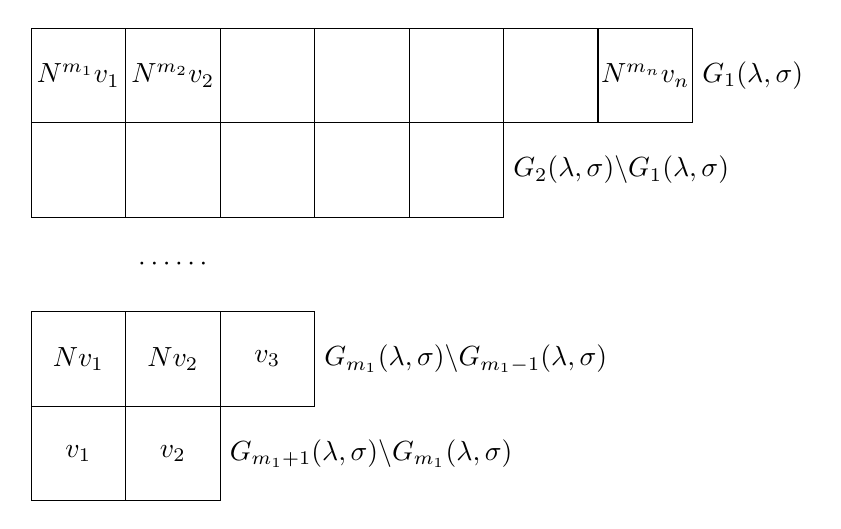
\begin{tikzpicture}[scale=1.2]
                  \foreach[count=\i] \len in {7, 7, 5, 3, 3, 2}
                  \draw (0, -\i+1) -- (\len, -\i+1);

                  \foreach \i in {0, 1, 2}
                  \draw (\i, -3) -- (\i, -5);

                  \draw (3, -3) -- (3, -4);

                  \foreach \i in {0,...,5}
                  \draw (\i, 0) -- (\i, -2);

                  \foreach \i in {6, 7}
                  \draw (\i, 0) -- (\i, -1);

                  \foreach \i in {1, 2} {
                  \node at (\i-.5, -4.5) {$v_{\i}$};
                  \node at (\i-.5, -.5) {$N^{m_{\i}}v_{\i}$};
                  }
                  \foreach \i in {1, 2}
                  \node at (\i-.5, -3.5) {$Nv_{\i}$};

                  \node at (3-.5, -3.5) {$v_{3}$};
                  \node at (6.5, -.5) {$N^{m_n}v_n$};
                  \node at (1.5, -2.5) {$\cdots\cdots$};

                  \node[anchor=west] at (7, -.5) {$G_1(\lambda,\sigma)$};
                  \node[anchor=west] at (5, -1.5) {$G_2(\lambda,\sigma) \backslash G_1(\lambda,\sigma)$};
                  \node[anchor=west] at (3, -3.5) {$G_{m_1}(\lambda,\sigma) \backslash G_{m_1-1}(\lambda,\sigma)$};
                  \node[anchor=west] at (2, -4.5) {$G_{m_1+1}(\lambda,\sigma) \backslash G_{m_1}(\lambda,\sigma)$};
              \end{tikzpicture}
              \caption{将若当基排列成Young图形式}
              \label{fig:17:若当基Young图形式}
          \end{figure}

    \item 接下来要确定每个若当循环基的长度，也就是Young图每一列的长度，我们应当从行的性质入手，因为这是我们目前仅有的可以计算的信息. 我们需要求解每个$G_j(\lambda,\sigma)$及其维数（目前只有维数有用，但后续求解具体若当基时其中的向量也是有用的），直到某个$G_j(\lambda,\sigma)$的维数等于$G_\lambda$的维数，因为Young图中所有方格与$G_\lambda$的一组基一一对应，因此方格总数就等于$G_\lambda$的维数. 另一方面由\autoref{thm:广义特征性质}，$N$是$G_\lambda$上的幂零线性变换，且在其它广义特征子空间上是双射，因此 $N$ 的各幂次的核空间最高维数也只能是$G_\lambda$的维数.

          在求出各个$G_j(\lambda,\sigma)$的维数后阶梯形状也即确定，因为各层向量个数确定了. 举个简单的例子，假设$G_\lambda$是11维空间，满足$G_1(\lambda,\sigma)$，$G_2(\lambda,\sigma)$，$G_3(\lambda,\sigma)$的维数分别为5,9,11. 对照Young图每行右侧的标注，这说明从最上方一行往下的向量个数依次为5，4($=9-5$)，2($=11-9$)，具体Young图为
          \begin{figure}[H]
              \centering
              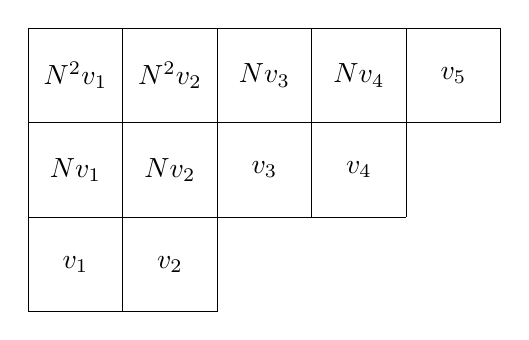
\begin{tikzpicture}[scale=1.2]
                  \foreach[count=\i] \len in {5, 5, 4, 2}
                  \draw (0, -\i+1) -- (\len, -\i+1);

                  \foreach \i in {0,...,5}
                  \draw (\i, 0) -- (\i, -1);
                  \foreach \i in {0,...,4}
                  \draw (\i, -1) -- (\i, -2);
                  \foreach \i in {0, 1, 2}
                  \draw (\i, -2) -- (\i, -3);

                  \node at (.5, -.5) {$N^2v_1$};
                  \node at (1.5, -.5) {$N^2v_2$};
                  \node at (2.5, -.5) {$Nv_3$};
                  \node at (3.5, -.5) {$Nv_4$};
                  \node at (4.5, -.5) {$v_5$};
                  \node at (.5, -1.5) {$Nv_1$};
                  \node at (1.5, -1.5) {$Nv_2$};
                  \node at (2.5, -1.5) {$v_3$};
                  \node at (3.5, -1.5) {$v_4$};
                  \node at (.5, -2.5) {$v_1$};
                  \node at (1.5, -2.5) {$v_2$};
              \end{tikzpicture}
          \end{figure}
          然后我们就能得到每组若当循环基的长度，即每个若当块的阶数，分别为$3,3,2,2,1$.
\end{enumerate}

基于上面的求解过程，我们就可以得到一般性的Young图大小的决定公式如下：
\begin{theorem}{}{Young图行长度}
    令$r_j$表示Young图从上至下第$j$行的格数，则有（其中$N=\sigma-\lambda I$）：
    \begin{enumerate}
        \item $r_1=\dim V-r(N)$；
        \item $r_j=r(N^{j-1})-r(N^j)(j>1)$.
    \end{enumerate}
\end{theorem}
\begin{proof}
    根据\autoref{fig:17:若当基Young图形式} 中每行右侧的标注的含义，第一行的格数就是$G_1(\lambda,\sigma)$的维数，即特征子空间的维数，即$\dim V-r(N)$；第$j(j>1)$行的格数就是$G_j(\lambda,\sigma)$的维数减去$G_{j-1}(\lambda,\sigma)$的维数，由线性映射基本定理，$\dim G_j(\lambda,\sigma)=\dim G_\lambda-r(N^j)$，$\dim G_{j-1}(\lambda,\sigma)=\dim G_\lambda-r(N^{j-1})$，因此第$j$行的格数就是$r(N^{j-1})-r(N^j)$.
\end{proof}

基于上述定理，我们可以进一步得到每个特征值对应的若当块个数和每个若当块大小的公式. 进一步地，这些公式实际上就表明了若当标准形的唯一性，因为每个特征值对应的若当块的个数和大小都可以被如下公式唯一确定. 我们将这一定理总结如下：
\begin{theorem}{}{若当标准形唯一}
    设$V$是$n$维复向量空间，$\sigma\in \mathcal{L}(V)$，$\lambda_1,\ldots,\lambda_m$为其互异的特征值，记$N_j=\sigma-\lambda_j I$，则主对角元为$\lambda_j$的若当块的个数$n_j$为
    \begin{equation} \label{eq:17:若当块个数}
        n_j=n-r(N_j),
    \end{equation}
    其中$t$级若当块$J_t(\lambda_j)$的个数$n_j(t)$为
    \begin{equation} \label{eq:17:若当块大小}
        n_j(t)=r(N_j^{t+1})+r(N_j^{t-1})-2r(N_j^t),
    \end{equation}
    以上公式表明，除若当块的排列次序外，一个线性变换对应的若当标准形唯一.
\end{theorem}
\begin{proof}
    实际上，证明这一定理就是要从\autoref{thm:Young图行长度} 中得到的Young图每行的长度推出Young图有多少列，以及每列的长度. 很显然，Young图的列数就是第一行的长度，即$\dim V-r(N_j)$. 进一步观察，我们知道Young图第$j$行与第$j+1$行的长度之差来源于有$r_j-r_{j+1}$（记号来源于\autoref{thm:Young图行长度}）组循环若当基长度终止于$j$，因此大小为$j$的若当块的个数就是$r_j-r_{j+1}=r(N_j^{t+1})+r(N_j^{t-1})-2r(N_j^t)$.
\end{proof}

尽管我们理论上可以通过上述过程得到任意复向量空间上的线性变换的若当块的个数和大小，但我们知道，直接对线性变换计算特征值是困难的，因此更多的时候我们仍然是利用线性变换和它的矩阵表示的特征值与广义特征向量的对应关系，将求解线性变换的若当标准形转化为求解其某个矩阵表示的若当标准形.

于是我们讨论矩阵的情况. 我们考虑$P^{-1}AP=J$，其中$P$为过渡矩阵，$J$为$A$的若当标准形. 我们可以将$A$视为$\sigma(\alpha)=A\alpha$在自然基下的矩阵，于是$\sigma$在\autoref{cor:若当基存在} 给出的基（记为$B$）下的表示矩阵的求解方式就是$\sigma(B)=(B)J$，将$B$组成的矩阵记作$P$，代入$\sigma$的定义，$\sigma(B)=(B)J$就等同于$AP=PJ$，即$P^{-1}AP=J$，故如果我们要求矩阵相似于其若当标准形的过渡矩阵，问题转化为求解$\sigma(\alpha)=A\alpha$的若当基然后排列成矩阵即可.

然而我们知道，求解$\sigma$的若当基需要求解各个$G_i(\lambda,\sigma)=\ker(\sigma-\lambda I)^i$，代入$\sigma(\alpha)=A\alpha$可知，$G_i(\lambda,\sigma)$实际上就是$(A-\lambda I)^iX=0$的解. 所以对于矩阵而言，上述所有的过程都只是不断对矩阵求幂然后解线性方程组，因此是一定可解的. 我们用解空间替代各个$G_i(\lambda,\sigma)$重复上述过程可以得到如下定理：
\begin{theorem}{}{矩阵若当标准形唯一}
    设$A$是$n$阶复矩阵，$\lambda_1,\ldots,\lambda_m$为其互异的特征值，则主对角元为$\lambda_j$的若当块的个数$n_j$为
    \begin{equation} \label{eq:17:矩阵若当块个数}
        n_j=n-r(A-\lambda_j E),
    \end{equation}
    其中$t$级若当块$J_t(\lambda_j)$的个数$n_j(t)$为
    \begin{equation} \label{eq:17:矩阵若当块大小}
        n_j(t)=r(A-\lambda_j E)^{t+1}+r(A-\lambda_j E)^{t-1}-2r(A-\lambda_j E)^t,
    \end{equation}
    以上公式表明，除若当块的排列次序外，一个矩阵对应的若当标准形唯一.
\end{theorem}

最后我们需要提到一点，根据上面的叙述，若当标准形在不考虑若当块的排列顺序的情况下是唯一的. 因此任一复数域上矩阵均有唯一的若当标准形（相似标准形），因此我们可以知道，两矩阵相似的一个充要条件是两矩阵有相同的若当标准形（不考虑若当块的排列顺序），这也是判定两个矩阵是否相似的关键，当然之后我们还会学到其它判定方式，届时我们再做总结.

接下来我们将讨论如何求出Young图中所有方格中的向量，当然实际上只需确定每个终止向量即可得到所有向量. 在正式讨论之前，我们先考虑一种投机取巧的方式. 事实上，如果题目只要求我们求解矩阵的若当标准形时，如果我们要求解过渡矩阵，也有简单的方法. 要求$P$使得$P^{-1}AP=J$，则有$AP=PJ$. 假定$P$为$n$阶矩阵，我们可以设$P=(X_1,\ldots,X_n)$，剩下的任务就是解方程了. 因此这种方法非常简单，缺陷在于绕开了若当基这一本质的问题.
\begin{example}{}{求若当标准形过渡矩阵}
    利用上述方法求解矩阵\[\begin{pmatrix}
            2 & 3 & 2 \\ 1 & 8 & 2 \\ -2 & -14 & -3
        \end{pmatrix}\]的若当标准形以及对应的过渡矩阵.
\end{example}

\begin{solution}
    记 $A=\begin{pmatrix}
        2 & 3 & 2 \\ 1 & 8 & 2 \\ -2 & -14 & -3
    \end{pmatrix}$，可以解得$A$的特征多项式为 $(\lambda-1)(\lambda-3)^2$，因此特征值为$1$和$3$，且$A-3E=\begin{pmatrix}
        -1 & 3 & 2 \\ 1 & 5 & 2 \\ -2 & -14 & -6
    \end{pmatrix}$的秩为$2$，因此$3$对应的若当块个数为$3-2=1$，结合\autoref{thm:矩阵若当标准形唯一}的结论不难得到若当标准型为$\begin{pmatrix}
        3 & 1 & 0 \\ 0 & 3 & 0 \\ 0 & 0 & 1
    \end{pmatrix}$.

    设过渡矩阵为$P=(X_1, X_2, X_3)$，则有$AP=PJ$，即
    \[
        \begin{cases}
            AX_1=3X_1 \\ AX_2=X_1+3X_2 \\ AX_3=X_3
        \end{cases}
    \]
    求解方程组 $AX=X$ 可得 $X_3=(2,0,-1)^\mathrm{T}$，求解方程组 $AX=3X$ 可得 $X_1=(1,-1,2)^\mathrm{T}$，将 $X_1$ 代入方程组 $AX=X_1+3X$ 可得 $X_2=(-1,0,0)^\mathrm{T}+k(1,-1,2)^\mathrm{T}$，取 $k=0$ 即可得到 $X_2=(-1,0,0)^\mathrm{T}$，因此过渡矩阵为
    \[P=\begin{pmatrix}
        1 & -1 & 2 \\ -1 & 0 & 0 \\ 2 & 0 & -1
    \end{pmatrix}.\]
\end{solution}

下面我们将讨论对于一般的线性变换，无法投机取巧时，或者希望从更本质的角度求解时，我们应当使用的方法.

\begin{center}
    \textbf{\heiti 第二步\quad 求解 $\boldsymbol{v_1,\ldots,v_n}$}
\end{center}

\begin{enumerate}
    \item 实际上，我们在前述求解若当块大小的过程中求出了各个$G_j(\lambda,\sigma)$，接下来我们需要利用这些向量将之前确定形状的阶梯内容填满. 我们首先确定Young图最后一行的向量，也就是 $G_{m_1+1}(\lambda,\sigma) \backslash G_{m_1}(\lambda,\sigma)$，其中 $G_{m_1+1}(\lambda,\sigma)$ 就是$V$，需要求出它和$G_{m_1}(\lambda,\sigma)$的差. 似乎很简单，但若仔细思索便会发现线性空间的差并不一定好求. 举一个简单的例子，设$G_{m_1+1}(\lambda,\sigma)=\{\alpha_1,\alpha_2,\alpha_3,\alpha_4\}$，$G_{m_1}(\lambda,\sigma)=\{\beta_1,\beta_2\}$. 这其中出现的所有向量可能都完全不一样，所以作差并不容易. 但我们有一种好方法，如果我们能从$G_{m_1+1}(\lambda,\sigma)$中挑选两个向量和$G_{m_1}(\lambda,\sigma)$中的两个向量放在一起，并且这四个向量线性无关，这就说明这两个挑出的向量就是作差的结果. 原因在于线性无关意味着$G_{m_1}(\lambda,\sigma)$与这两个向量构成的空间作和为直和，考虑维数即可知得到的是$G_{m_1+1}(\lambda,\sigma)$. 而要找到这样的向量，可以参考\autoref{lem:极大线性无关组的求法} 后续讨论中求一组线性无关向量扩张成一组基的方法，实际上扩张进来的向量就是作差的结果.

    \item 接下来继续计算倒数第二行中的向量. 实际上算出倒数第一行后倒数第二行中部分向量就已经确定了，例如\autoref{fig:17:若当基Young图形式} 上的$Nv_1$和$Nv_2$. 我们这时用类似的方法求解$G_{m_1}(\lambda,\sigma)$和$G_{m_1-1}(\lambda,\sigma)$的差，但新选出的向量除了需要和$G_{m_1-1}(\lambda,\sigma)$中的向量线性无关以外，还需要和同一行中已经求出的向量（$Nv_1,Nv_2$）线性无关，因此可以将这两部分向量合并成一个集合，求它和 $G_{m_1}(\lambda,\sigma)$ 的差即可，步骤和之前一样.

          这其实不局限于倒数第二行，对于任意的 $1 \leqslant j \leqslant m_1$，处于$G_j(\lambda,\sigma)\backslash G_{j-1}(\lambda,\sigma)$对应的行的需要补充的向量$v$应当满足如下三个条件：
          \begin{enumerate}
              \item $v\in G_j(\lambda,\sigma)$；

              \item $v\notin G_{j-1}(\lambda,\sigma)$；

              \item $v$与同一行中左边已求出的向量线性无关.
          \end{enumerate}

    \item 最后，我们将所有求出的基按照若当基原先的排列顺序重新组合即可. 如果求矩阵相似于若当标准形的过渡矩阵，则按顺序按列摆放即可.
\end{enumerate}

我们可以通过一个例子来说明上述过程.
\begin{example}{}{}
    设$V$是由两个变量$x,y$生成的次数不大于2的多项式函数（例如$xy^2$不是，因为次数等于1+2=3，$x^2+y$是）关于一般的多项式加法和数乘构成的线性空间，于是我们可以取一组基为$\{1,x,y,x^2,y^2,xy\}$，定义$\sigma\in \mathcal{L}(V)$为
    \[\sigma(f(x,y))=\dfrac{\partial}{\partial x}f(x,y).\]
    求$V$的一组基使得$\sigma$在这组基下的矩阵是若当标准形.
\end{example}
\begin{solution}
    由于对多项式求导会降低次数，因此$\sigma$显然是幂零的（也可以直接写出$\sigma$在题目中给出的这组基的矩阵表示，不难得知其为对角线全为$0$的上三角矩阵），因此唯一特征值为$0$. 为了表示简便，这里用 $G_j$ 代替之前的记号 $G_j(\lambda,\sigma)=\ker (\sigma-\lambda I)^j$.

    不难得到：
    \begin{itemize}
        \item $G_1 = \ker \sigma = \spa\{1, y, y^2\}$，$\dim G_1 = 3$；
        \item $G_2 = \ker \sigma^2 = \spa\{1, y, y^2, x, xy\}$，$\dim G_2 = 5$；
        \item $G_3 = \ker \sigma^3 = \spa\{1, y, y^2, x, xy, x^2\} = V$，$\dim G_3 = 6$.
    \end{itemize}

    从而根据\autoref{thm:Young图行长度}，Young图的行长度分别为 $r_1 = 3, r_2 = 2, r_3 = 1$，我们按照刚刚的讨论填充Young图.

    \begin{enumerate}
        \item 倒数第一层中，我们需要找到一个向量 $v_1 \in G_3 \backslash G_2$，因为这里$G_1, G_2, G_3$的基满足了包含关系，所以作差变得非常简单：直接挑出 $v_1=x^2$ 即可.
        \item 倒数第二层中，我们需要找到一个向量 $v_2 \in G_2 \backslash G_1$，且 $v_2$ 与该层已有向量 $\sigma(v_1)=2x$ 线性无关. 注意到 $G_2 = \spa\{G_1, x, xy\}$，在 $G_2$ 中，$\{1, y, y^2, 2x, xy\}$ 线性无关且张成 $G_2$，故可取 $v_2 = xy$.
        \item 第一层中，我们需要找到一个向量 $v_3 \in G_1$，且 $v_3$ 与该层已有向量 $\sigma^2(v_1)=2, \sigma(v_2)=y$ 线性无关. 注意到 $G_1 = \spa\{1, y, y^2\}$. 显然 $\{2, y, y^2\}$ 是 $G_1$ 的一组基，故可取 $v_3 = y^2$.
    \end{enumerate}

    从而我们得到了若当基 $\{2, 2x, x^2, y, xy, y^2\}$.
\end{solution}

\section{若当标准形的应用}
\subsection{求解不变子空间}
在不变子空间一节中我们提到，我们可以利用若当标准形求解不变子空间. 下面是一个与若当块直接相关的例子：
\begin{example}{}{}
    设$V$为$n$维复向量空间，$\sigma\in \mathcal{L}(V)$，$\sigma$在基$v_1,\ldots,v_n$下的矩阵是一个若当块
    \[\begin{pmatrix}
            \lambda & 1       & 0      & \cdots & 0       \\
            0       & \lambda & 1      & \cdots & 0       \\
            \vdots  & \vdots  & \vdots & \ddots & \vdots  \\
            0       & 0       & 0      & \cdots & \lambda
        \end{pmatrix},\]
    证明：
    \begin{enumerate}
        \item $V$中包含$v_n$的不变子空间只有$V$自身；

        \item $V$中任意非零不变子空间都包含$v_1$；

        \item $V$不能分解为两个非平凡的不变子空间的直和；

        \item $V$中有且仅有$n+1$个不变子空间，它们分别是
              \[\{0\},\spa(v_1),\spa(v_1,v_2),\ldots,\spa(v_1,\ldots,v_{n-1},v_n)\]
    \end{enumerate}
\end{example}

\begin{solution}
    \begin{enumerate}
        \item 设$W$是包含$v_n$的不变子空间，根据线性映射矩阵表示的定义，$\sigma(v_n)=\lambda v_n+v_{n-1}\in W$，故$v_{n-1}\in W$，同理可得$v_{n-2},\ldots,v_1\in W$，即$W=V$.

        \item 设$U$为任一非零不变子空间，那么$U$中存在一个非零向量$v$，则$v$一定可以表达为
              \[v=k_1v_1+\cdots+k_sv_s(s\leqslant n),\]
              其中$k_s\neq 0$. 由$\sigma(v)\in U$以及线性映射矩阵表示有
              \begin{align*}
                  \sigma(v) & = \lambda k_1v_1+k_2(\lambda v_2+v_1)+\cdots+k_s(\lambda v_s+v_{s-1}) \\
                            & = \lambda v+k_2v_1+\cdots+k_sv_{s-1}\in U,
              \end{align*}
              因此$k_2v_1+\cdots+k_sv_{s-1}\in U$，同理进一步作用$\sigma$有$k_3v_1+\cdots+k_sv_{s-2}\in U$，以此类推有$k_sv_1\in U$. 又$k_s\neq 0$，故$v_1\in U$，命题得证.

        \item 利用上一点显然.

        \item 显然$\{0\},\spa(v_1),\spa(v_1,v_2),\ldots,\spa(v_1,\ldots,v_{n-1},v_n)$都是不变子空间，下面证明不变子空间一定在它们当中.

              设$U$为任一不变子空间，若$U=\{0\}$，则也符合结论. 我们考虑非零的情况，设$\beta_1,\ldots,\beta_s$是$U$的一组基，并且假设
              \[\beta_i=a_{i1}v_1+a_{i2}v_2+\cdots+a_{it}v_t,\enspace i=1,2,\ldots,s\]
              其中满足至少有一个$i$使得$a_{it}\neq 0$（把所有基下表示末尾的0去除即可）. 对于满足$a_{it}\neq 0$的$i$，由于$U$是不变子空间，故$\sigma(\beta_i)\in U$，与第二点证明完全相同，我们得到
              \begin{align*}
                  a_{i2}v_1+a_{i3}v_2+\cdots+a_{it}v_{t-1}\in U, \\
                  a_{i3}v_1+a_{i4}v_2+\cdots+a_{it}v_{t-2}\in U, \\
                  \cdots                                         \\
                  a_{i,t-1}v_1+a_{it}v_2\in U,                   \\
                  a_{it}v_1\in U.
              \end{align*}
              由于$a_{it}\neq 0$，故由最后的式子知道$v_1\in U$. 代入倒数第二个式子知道$v_2\in U$，以此类推，最终得到$\spa(v_1,\ldots,v_t)\subset U$，而$U\subset\spa(v_1,\ldots,v_t)$显然（因为每个$\beta_i$都在其中），故命题得证.
    \end{enumerate}
\end{solution}

因此我们如果能将线性变换在一组基下表示为若当块，我们就可以很快地利用这一例子的结论写出其不变子空间. 但我们有时候会遇到线性变换在一组基下表示为多个若当块的情况，这时我们可能需要通过组合不同若当块对应的不变子空间来得到线性变换的不变子空间（很容易知道不相交的不变子空间的直和还是不变子空间，因为矩阵表示还是分块对角矩阵），并且同时还要证明组合出来的就是全部的不变子空间. 下面就是一个非常经典的例子：
\begin{example}{}{}
    设$V$是复数域上的$n$维线性空间，$\sigma\in\mathcal{L}(V)$，若$\sigma$有$n$个不同的特征值$\lambda_1,\ldots,\lambda_n$，求$\sigma$的不变子空间的个数.
\end{example}
\begin{solution}
    显然$\sigma$可对角化，每个对角元素就是一阶若当块，因此我们需要考虑组合这些若当块对应的基构成新的不变子空间. 由可对角化我们有
    \[V=V_{\lambda_1}\oplus\cdots\oplus V_{\lambda_n},\]
    结合$\dim V=n$可知每个特征子空间都是1维的. 根据我们组合的思想，我们知道对于任意的$1\leqslant j_1<j_2<\cdots<j_r\leqslant n$，$r=1,2,\ldots,n$，$V_{\lambda_{j_1}}\oplus\cdots\oplus V_{\lambda_{j_r}}$都是不变子空间. 这样的不变子空间加上零空间的个数总和为$\mathrm{C}_n^0+\mathrm{C}_n^1+\cdots+\mathrm{C}_n^n=2^n$.

    下面我们需要说明这些不变子空间是全部的不变子空间. 设$U$为任一不变子空间，若为零空间则符合要求，若不是零空间，设$\dim U=m>0$，$U$的一组基为$\beta_1,\ldots,\beta_m$，将其扩充为$V$的一组基$\beta_1,\ldots,\beta_m,\beta_{m+1},\ldots,\beta_n$，则在这组基下$\sigma$的矩阵为
    \[B=\begin{pmatrix}
            A & C \\ O & D
        \end{pmatrix},\]
    于是$\sigma\vert_U$的矩阵为$A$，对应特征多项式$|\lambda E-A|$，而$\sigma$的特征多项式$|\lambda E-B|=|\lambda E-A||\lambda E-D|$. 由于$\sigma$有$n$个不同的特征值，因此$\sigma\vert_U$必定有$m$个不同的特征值$\lambda_{l_1},\ldots,\lambda_{l_m}$，且$1\leqslant l_1<\cdots<l_m\leqslant n$. 而对每个特征值$\lambda_{l_i}$都有特征向量$\alpha_i\in U$，满足$\sigma\vert_U(\alpha_i)=\lambda_{l_i}\alpha_i$，因此$\sigma(\alpha_i)=\lambda_{l_i}\alpha_i$，即$\alpha_i\in V_{\lambda_{l_i}}$，故$V_{\lambda_{l_1}}\oplus\cdots\oplus V_{\lambda_{l_m}}\subset U$. 再结合
    \[\dim(V_{\lambda_{l_1}}\oplus\cdots\oplus V_{\lambda_{l_m}})=m=\dim U,\]
    故$U=V_{\lambda_{l_1}}\oplus\cdots\oplus V_{\lambda_{l_m}}$，故所有不变子空间都是之前讨论的$2^n$种之一，命题得证.
\end{solution}

当然需要注意的是，不变子空间的个数不一定有限，例如对于数乘变换$\sigma=kI\in\mathcal{L}(V)$，很容易验证$V$的任意子空间都是其不变子空间.

\subsection{矩阵求幂与马尔可夫链}

若当标准形的另一个应用在于我们可以利用它计算矩阵的幂，因为若当块的幂的计算是简单的，这一点与对角矩阵是类似的：
\begin{equation} \label{eq:若当块幂}
    J_k(a)^n=(aE+J_k(0))^n=a^nE+\mathrm{C}_n^1a^{n-1}J_k(0)+\cdots+\mathrm{C}_n^nJ_k(0)^n.
\end{equation}
同时我们也知道$J_k(0)^k=O$（幂零矩阵），并且通过简单的找规律不难找到$J_k(0)$的任意次幂的表达式，所以利用若当标准形求解矩阵的幂是简单的. 我们来看一个例子：
\begin{example}{}{}
    设$A=\begin{pmatrix}
            2 & 6 & -15 \\ 1 & 1 & -5 \\ 1 & 2 & -6
        \end{pmatrix}$，求$A^{m}(m\geqslant 1)$.
\end{example}
\begin{solution}
    首先求 $A$ 的若当标准形，$|\lambda E - A|=(\lambda + 1)^3$，$-1$为唯一特征值，几何重数为$3$，而$A+E=\begin{pmatrix}
            3 & 6 & -15 \\ 1 & 2 & -5 \\ 1 & 2 & -5
        \end{pmatrix}$为秩为$1$的矩阵，因此由\autoref{thm:矩阵若当标准形唯一}，若当块有$3-1=2$个，只可能是$J_2(-1)$和$J_1(-1)$，因此$A=PJP^{-1}$，其中$J=\begin{pmatrix}
            -1 & 1 & 0 \\ 0 & -1 & 0 \\ 0 & 0 & -1
        \end{pmatrix}$，用\autoref{ex:求若当标准形过渡矩阵} 中的方法，可得$P=\begin{pmatrix}
            3 & 1 & 2 \\ 1 & 0 & -1 \\ 1 & 0 & 0
        \end{pmatrix}$，$P^{-1}=\begin{pmatrix}
            0 & 0 & 1 \\ 1 & 2 & -5 \\ 0 & -1 & 1
        \end{pmatrix}$，故$A^m=PJ^mP^{-1}$，其中
        \[
            J^m=\begin{pmatrix}
                (-1)^m E + m(-1)^{m-1}J_2(0) & O \\ O & (-1)^m
            \end{pmatrix}=(-1)^m\begin{pmatrix}
                1 & -m & 0 \\ 0 & 1 & 0 \\ 0 & 0 & 1
            \end{pmatrix},
        \]
        整理可得 $A^m=(-1)^m\begin{pmatrix}
            1-3m & -6m & 15m \\ -m & 1-2m & 5m \\ -m & -2m & 1+5m
        \end{pmatrix}$.
\end{solution}

下面是一个非常经典的例子，在接下来的讨论中还会有应用：
\begin{example}{}{若当m次幂}
    设$J=J_n(a)$是特征值为$a$的$n$阶若当块，求$J^m$的若当标准形，其中$m$为非零整数.
\end{example}
\begin{solution}
    我们需要分别考虑$a\neq 0$和$a=0$的情况：
    \begin{enumerate}
        \item 当$a\neq 0$时，首先显然$J^m$的特征值都为$a^m$，我们先处理$m\geqslant 1$的情况，我们有
              \[J^m=(aE+J(0))^m=a^mE+\mathrm{C}_m^1a^{m-1}J_n(0)+\cdots+\mathrm{C}_m^mJ_n(0)^m.\]
              故$r(J^m-a^mE_n)=r(\mathrm{C}_m^1a^{m-1}J_n(0)+\cdots+\mathrm{C}_m^mJ_n(0)^m)=n-1$（很容易通过$J_n(0)$的幂次的特点写出这一矩阵，然后通过行列式秩判断），因此根据\autoref{thm:若当标准形唯一} 可知$J^m$的若当块个数为$n-(n-1)=1$，因此$J^m$的若当标准形就是$J_n(a^m)$.

              然后我们考虑$m=-1$的情况，显然$J^{-1}$的特征值为$a^{-1}$，这里我们借用\autoref{ex:分式求逆1} 的分式思想，得到
              \[J^{-1}=\dfrac{1}{a}E_n-\dfrac{1}{a^2}J_n(0)+\cdots+(-1)^{n-1}\dfrac{1}{a^n}J_n(0)^{n-1}.\]
              故$r(J^{-1}-\dfrac{1}{a}E_n)=r(-\dfrac{1}{a^2}J_n(0)+\cdots+(-1)^{n-1}\dfrac{1}{a^n}J_n(0)^{n-1})=n-1$，因此$J^{-1}$的若当块个数为$n-(n-1)=1$，因此$J^{-1}$的若当标准形就是$J_n(a^{-1})$.

              最后处理$m\leqslant -2$的情况，注意到$J^m=(J^{-1})^{-m}$，故根据前面$m\geqslant 1$的讨论，$J^m$的若当标准形就是$J_n((a^{-1})^{-m})=J_n(a^m)$.

              综上所述，无论$m$取什么整数值，$J^m$的若当标准形就是$J_n(a^m)$.

        \item 当$a=0$时，$J$不可逆，因此只考虑$m>0$的情形. 我们有$m\geqslant n$时$J^m=O$，此时若当标准形也就是零矩阵. 我们考虑$m<n$的情况，我们需要使用\autoref{thm:若当标准形唯一} 的结论来辅助我们求解$J^m$的若当标准形，因此我们需要研究$(J^m)^k$的秩. 我们做带余除法，$n=mq+r(0\leqslant r<m)$，则根据$J_n(0)$的幂次的特点，我们有
              \[r((J^m)^k)=n-mk,\enspace 0\leqslant k\leqslant q,\enspace r((J^m)^k)=0,\enspace k\geqslant q+1.\]
              因此
              \begin{enumerate}
                  \item $1\leqslant k<q$时，$J_k(0)$的个数为$r((J^m)^{k-1})+r((J^m)^{k+1})-2r((J^m)^k)=(n-m(k-1))+(n-m(k+1))-2(n-mk)=0$；
                  \item $k=q$时，$J_k(0)$的个数为$r((J^m)^{q-1})+r((J^m)^{q+1})-2r((J^m)^q)=(n-m(q-1))+0-2(n-mq)=m-r$；
                  \item $k=q+1$时，$J_k(0)$的个数为$r((J^m)^q)+r((J^m)^{q+2})-2r((J^m)^{q+1})=(n-mq)+0-0=r$.
                  \item $k>q+1$时，$J_k(0)$的个数为0.
              \end{enumerate}
              综上所述，$J^m$的若当标准形是$\diag(J_q(0),\ldots,J_q(0),J_{q+1}(0),\ldots,J_{q+1}(0))$，其中$J_q(0)$的个数为$m-r$，$J_{q+1}(0)$的个数为$r$.
    \end{enumerate}
\end{solution}

由于复数域上任意矩阵都有若当标准形，因此利用若当标准形，我们可以求出复数域上任意矩阵的任意幂次. 于是我们会有一个问题，即任意给定一个矩阵，当我们取其幂次趋向于无穷时，会得到一个什么样的矩阵呢？是所有元素都有限的矩阵，还是有些元素可能趋于无穷了呢？

这个问题可以用若当标准形回答. 事实上，矩阵幂是否收敛（这里将矩阵的收敛定义为矩阵的每个元素都收敛）取决于各个若当块在高次幂下的行为. 基于\autoref{ex:若当m次幂} 的结果，直观而言这取决于特征值（可能为复数）$\lambda$的模长. 下面我们将给出一个严格的判别条件.

\begin{theorem}{}{矩阵幂收敛判别}
    设$A\in\mathbf{C}^{n\times n}$，并设$A$的若当标准形为 $J=\diag(J_{r_1}(\lambda_1),J_{r_2}(\lambda_2),\ldots,J_{r_s}(\lambda_s))$，则 $\{A^m\}_{m\geqslant 1}$收敛当且仅当 $A$ 的每一个若当块都满足下列两种情形之一：
    \begin{enumerate}
        \item 该若当块的特征值$\lambda$满足$|\lambda|<1$；
        \item 该若当块恰为$J_1(1)$.
    \end{enumerate}
\end{theorem}

\begin{proof}
    先讨论单个若当块$J_k(\lambda)$的情形. 根据\autoref{ex:若当m次幂} 的结果，有
    \begin{enumerate}
        \item 若$|\lambda|<1$，则 $J_k(\lambda)^m\to O$，因此收敛于零矩阵（注意 $P^{-1}AP$ 的每个元素是 $A$ 各元素的固定线性组合）.

        \item 若$|\lambda|>1$，则$J_k(\lambda)^m$的对角元都是 $\lambda^m$，从而不可能收敛.

        \item 若$|\lambda|=1$ 且 $k\geqslant 2$，根据\autoref{eq:若当块幂}，$J_k(\lambda)^m$的第一条超对角线上的元素为$\mathrm{C}_m^1\lambda^{m-1}=m\lambda^{m-1}$，其模长等于$m$，故不可能收敛.

        \item 若$|\lambda|=1$ 且 $k=1$，则$J_1(\lambda)^m=\lambda^m$. 这一数列收敛当且仅当$\lambda=1$；事实上，若$\lambda^m\to l$，则$\lambda^{m+1}\to l$，于是$\lambda^{m+1}-\lambda^m\to 0$，即$\lambda^m(\lambda-1)\to 0$. 取模后得$|\lambda-1|=|\lambda^m(\lambda-1)|\to 0$，故$\lambda=1$.
    \end{enumerate}

    综上，一个若当块的幂次收敛，当且仅当它要么对应于模长严格小于$1$的特征值，要么恰好是$J_1(1)$.

    再看一般矩阵$A$. 由$A^m=PJ^mP^{-1}$可知，$\{A^m\}$收敛当且仅当$\{J^m\}$收敛；而$J^m$是各若当块幂次构成的分块对角矩阵，因此$\{J^m\}$收敛当且仅当每个若当块的幂次都收敛. 于是便得到定理中的判别条件.
\end{proof}

等价地，上述定理给出的条件也可以写为：$\{A^m\}_{m\geqslant 1}$收敛，当且仅当（1）$A$的全部特征值都满足$|\lambda|\leqslant 1$；（2）若$|\lambda|=1$，则必有$\lambda=1$；（3）特征值$1$对应的全部若当块都是$1$级若当块. 若上述条件成立，并且特征值 $1$ 对应的 $1$ 级若当块共有 $r$ 个，则经过重新排列若当块后可写成 $J=\diag(I_r,J_0)$，其中$J_0$的全部特征值都满足 $|\lambda| < 1$，并且 $\lim_{m\to\infty}A^m=P\diag(I_r,O)P^{-1}$. 也就是说，当极限存在时，这个极限矩阵实际上就是投影到特征值 $1$ 对应特征子空间上的投影矩阵. 对于实矩阵，只需将它视为复矩阵后应用同样的判别，因为矩阵幂是否收敛并不因系数域扩张到复数域而改变.

这一定理在概率论中有一个非常经典的应用，这就是有限状态马尔可夫链. 所谓马尔可夫链，就是下一步所处的状态只依赖于当前状态，而与更早的历史无关的随机过程. 一个经典的例子是天气预测：

\begin{example}{}{}
    设某地的天气状态集合为$\{\text{晴},\text{阴},\text{雨}\}$，每天的天气状态只依赖于前一天的天气状态，并且满足如下转移概率：
    \begin{center}
        \begin{tabular}{c|ccc}
            & 晴   & 阴   & 雨   \\ \hline
            晴 & 0.5  & 0.3  & 0.2  \\
            阴 & 0.2  & 0.5  & 0.3  \\
            雨 & 0.1  & 0.4  & 0.5
        \end{tabular}
    \end{center}
    也就是说，如果前一天是晴，那么第二天是晴、阴、雨的概率分别为 $0.5, 0.3, 0.2$，其余类推.
\end{example}

下面开始形式化定义. 若状态集合为$\{1,2,\ldots,n\}$，并记$p_{ij}$为从状态$i$一步转移到状态$j$的概率，则得到转移矩阵
\[P=(p_{ij}),\qquad p_{ij}\geqslant 0,\qquad \sum_{j=1}^np_{ij}=1,\enspace i=1,2,\ldots,n.\]
这样的矩阵称为\term{随机矩阵}，更准确地说，这里是\term{行随机矩阵}，因为矩阵每一行的元素和为 $1$. 若初始时刻的状态分布写成概率行向量$\mu^{(0)}=(\mu_1^{(0)},\ldots,\mu_n^{(0)})$，则一步之后的分布为$\mu^{(1)}=\mu^{(0)}P$，进一步归纳可得$\mu^{(m)}=\mu^{(0)}P^m$. 因此，研究马尔可夫链经过很多步之后会趋向什么分布，本质上就是研究随机矩阵$P$的幂次$P^m$是否收敛以及收敛到什么矩阵.

\begin{corollary}{}{随机矩阵幂次收敛}
    设$P=(p_{ij})\in\mathbf{R}^{n\times n}$是一个行随机矩阵，则
    \begin{enumerate}
        \item $1$一定是$P$的特征值，并且$P$的任一特征值$\lambda$都满足$|\lambda|\leqslant 1$；
        \item $\{P^m\}_{m\geqslant 1}$收敛，当且仅当$1$是$P$在单位圆上的唯一特征值，也就是说，对任意满足$\lambda\neq 1$的特征值都有$|\lambda|<1$.
    \end{enumerate}
    若上述条件成立，则极限矩阵仍是随机矩阵，并且是$P$在特征值$1$对应特征子空间上的投影.
\end{corollary}

\begin{proof}
    记$e=(1,1,\ldots,1)^\mathrm{T}$. 由于$P$ 每行元素和都为$1$，故$Pe=e$，因此$1$是$P$的特征值. 再由Gershgorin 圆盘第一定理（\autoref{thm:Gershgorin disks theorem}），$P$的每个特征值都落在某个圆盘
    \[D_i=\left\{z\in\mathbf{C}\mid |z-p_{ii}|\leqslant \sum_{j\neq i}p_{ij}\right\}=\{z\in\mathbf{C}\mid |z-p_{ii}|\leqslant 1-p_{ii}\}\]
    中. 对于任意$z\in D_i$，由三角不等式有 $|z|\leqslant |z-p_{ii}|+p_{ii}\leqslant 1$，因而$P$的全部特征值都满足$|\lambda|\leqslant 1$.

    又因为行随机矩阵的乘积仍是行随机矩阵，所以 $P^m$（$m\geqslant 1$）仍是行随机矩阵. 特别地，它的每个元素都落在区间$[0,1]$内. 因此矩阵序列 $\{P^m\}$ 的每个元素都是有界的，于是对任意可逆矩阵 $S$，矩阵 $S^{-1}P^mS$ 的每个元素也都是 $P^m$ 各元素的固定线性组合，从而仍有界. 设 $P = SJS^{-1}$ 是 $P$ 的若当标准形. 若 $J$ 中存在某个对应于 $|\lambda| = 1$ 的高阶若当块 $J_k(\lambda)$（其中 $k \geqslant 2$），那么由\autoref{eq:若当块幂}，$J_k(\lambda)^m$ 第一条超对角线上的元素为 $m\lambda^{m-1}$，其模长等于 $m$，从而 $\{J^m\}$ 必有元素无界. 这与 $\{J^m\}=\{S^{-1}P^mS\}$ 各元素有界矛盾. 因此，随机矩阵在单位圆上的特征值都只能对应 $1$ 级若当块. 根据\autoref{thm:矩阵幂收敛判别}，$\{P^m\}$ 收敛当且仅当单位圆上的特征值只有 $1$，这就证明了前两点.

    若 $\{P^m\}$ 收敛到某个矩阵 $L$，则 $L$ 显然是行随机矩阵的极限，因此仍是行随机矩阵. 又由\autoref{thm:矩阵幂收敛判别}，$L$ 正是 $P$ 在特征值 $1$ 对应特征子空间上的投影.
\end{proof}

例如$P=\begin{pmatrix}
        0 & 1 \\
        1 & 0
    \end{pmatrix}$对应一个在两个状态之间来回切换的马尔可夫链. 此时$P$的特征值为$1$与$-1$，因为单位圆上除了$1$之外还出现了$-1$，所以$P^m$不收敛，这恰好对应于该链始终带有周期性的振荡.

\subsection{若当标准形与矩阵分解}
矩阵分解是讨论标准形时绕不开的话题. 接下来我们讨论若当标准形在矩阵分解中的应用，先从矩阵方根问题开始. 下面的结论是前文线性变换平方根问题的自然延续：
\begin{theorem}{}{若当标准形m次根}
    设$m\geqslant 2$为整数. 在复数域上有如下关于若当块方根的结论：
    \begin{enumerate}
        \item 设$a\neq 0$，则存在矩阵$A$使得$A^m=J_n(a)$；
        \item 当$n\geqslant 2$时，不存在矩阵$A$使得$A^m=J_n(0)$.
    \end{enumerate}
\end{theorem}

\begin{proof}
    \begin{enumerate}
        \item 根据\autoref{ex:若当m次幂}，若$b\neq 0$，则$J_n(b)^m\sim J_n(b^m)$. 取$b\in\mathbf{C}$使得$b^m=a$，则$J_n(b)^m\sim J_n(a)$，因此存在可逆矩阵$P$使得$P^{-1}J_n(b)^mP=J_n(a)$. 令$A=P^{-1}J_n(b)P$，便有$A^m=J_n(a)$.

        \item 反证法. 若存在矩阵$A$使得$A^m=J_n(0)$，则$A$显然也为$n$阶幂零矩阵，因此有$A^n=O$（因此至少有$m\leqslant n$）. 设$n=mq-r(m\geqslant 2,0\leqslant r<m)$，则$O=A^{n+r}=(A^m)^q=J_n(0)^q\neq O$，这是因为$J_n(0)$至少需要$n$次才能化零，但$n=mq-r(m\geqslant 2,0\leqslant r<m)$表明$q<n$，故矛盾.
    \end{enumerate}
\end{proof}

由此可以重新证明\autoref{thm:幂零平方根} 的\ref*{item:16:幂零平方根:2}：复数域上的可逆线性变换一定有平方根，我们现在可以使用若当标准形的方式证明. 只需证明矩阵版本，因为基固定的情况下矩阵和线性映射一一对应. 设可逆变换对应可逆复矩阵$A$，则$A$的若当标准形$J$中每个若当块的特征值均非零. 根据上一定理，每个若当块都有平方根，故$J$有平方根，记为$B$，即$B^2=J$. 若$P^{-1}AP=J$，取$C=PBP^{-1}$，则$C^2=PB^2P^{-1}=PJP^{-1}=A$，故我们找到了任意可逆矩阵对应的平方根$C$. 这一结论显然可以进一步推广，即任意复数域上的可逆线性变换和可逆矩阵一定有$m$次方根.

若当标准形还可以导出著名的Jordan-Chevalley分解. 这一证明也展示了利用若当标准形证明一般矩阵性质的常用范式：
\begin{enumerate}
    \item 证明结论对于若当块成立；
    \item 证明结论对于若当标准形成立；
    \item 利用问题在相似下的不变性证明结论对于一般矩阵成立.
\end{enumerate}

上面对复可逆矩阵方根的讨论正是这一范式的例子：先证明非零特征值的若当块有方根，再推广到若当标准形，最后通过相似变换得到一般可逆矩阵的结论. 总而言之，当我们希望使用若当标准形证明矩阵具有的性质时，这些性质在相似下要有一定的不变性，然后遵照上述范式即可给出证明. 这也体现出研究相似标准形的一个重要意义：通过研究形式简单的相似标准形的良好性质，结合研究性质的相似不变性，即可通过研究更容易处理的相似标准形来研究一般矩阵的性质. 接下来我们证明这一著名的分解：

\begin{theorem}{Jordan-Chevalley分解}{}
    设$A$是$n$阶复矩阵，则$A$可分解为$A=B+C$，其中$B,C$满足如下条件：
    \begin{enumerate}
        \item $B$是可对角化的；
        \item $C$是幂零的；
        \item $BC=CB$；
        \item $B,C$均可以表示为$A$的多项式.
    \end{enumerate}
    不仅如此，满足上述条件1-3的分解是唯一的.
\end{theorem}

\begin{proof}
    先证明存在性. 首先从若当块入手，对于若当块$J_n(a)=aE_n+J_n(0)$，取$B=aE_n, C=J_n(0)$，则$B$可对角化，$C$幂零，且$BC=CB$. 又因为$C^n=(J_n(a)-B)^n$，故取$f(x)=(x-a)^n+a$，则
    \[
        f(J_n(a))=(J_n(a)-aE_n)^n+aE_n=aE_n=B.
    \]
    因此$B$可表示为$J_n(a)$的多项式，$C=J_n(a)-B$也可表示为$J_n(a)$的多项式.

    接下来推广到若当标准形$J$. 设$J$的互异特征值为$\lambda_1,\ldots,\lambda_m$，特征值$\lambda_i$对应$s_i$个若当块. 将$J$表示为
    \[J=\begin{pmatrix}
            J_{11} &        &          &        &        &        &          \\
                   & \ddots &          &        &        &        &          \\
                   &        & J_{1s_1} &        &        &        &          \\
                   &        &          & \ddots &        &        &          \\
                   &        &          &        & J_{m1} &        &          \\
                   &        &          &        &        & \ddots &          \\
                   &        &          &        &        &        & J_{ms_m}
        \end{pmatrix}.\]
    对每个$J_{ij}$，设若当块大小为$k_{ij}$. 类似于前面对若当块的讨论，对每个若当块取$M_{ij}=\lambda_i E_{k_{ij}}, N_{ij}=J_{k_{ij}}(0)$，并按$J$中若当块的顺序排列成分块对角矩阵$M,N$，则$J=M+N$，$M$可对角化，$N$是幂零的，且$MN=NM$容易验证.

    设特征值$\lambda_i$对应的最大若当块阶数为$k_i$，则对所有$j$都有$(J_{ij}-\lambda_iE_{k_{ij}})^{k_i}=O$. 由于$(x-\lambda_1)^{k_1},\ldots,(x-\lambda_m)^{k_m}$两两互素，由\nameref{thm:中国剩余定理}，存在多项式$f(x)$满足
    \[
        f(x)\equiv \lambda_i \pmod{(x-\lambda_i)^{k_i}},\enspace i=1,\ldots,m.
    \]
    因而存在多项式$g_i(x)$使得
    \[
        f(x)=g_i(x)(x-\lambda_i)^{k_i}+\lambda_i.
    \]
    代入$J_{ij}$可得
    \[
        f(J_{ij})=g_i(J_{ij})(J_{ij}-\lambda_iE_{k_{ij}})^{k_i}+\lambda_iE_{k_{ij}}
        =M_{ij}.
    \]
    故$f(J)=M$，于是$N=J-M=J-f(J)$也是$J$的多项式.

    接下来考虑一般情形，对一般矩阵$A$，取可逆矩阵$P$使得$P^{-1}AP=J$. 由$J=M+N$可得
    \[
        A=PJP^{-1}=PMP^{-1}+PNP^{-1}.
    \]
    令$B=PMP^{-1}$，$C=PNP^{-1}$. 相似变换保持可对角化、幂零性与乘法交换性，因此$B$可对角化，$C$幂零，且$BC=CB$. 又
    \[
        B=Pf(J)P^{-1}=f(PJP^{-1})=f(A),
    \]
    故$B$是$A$的多项式，$C=A-B$也是$A$的多项式.

    最后证明唯一性. 假设$A$有另一满足1-3的分解$A=B'+C'$，则$B-B'=C'-C$，由$B'C'=C'B'$，结合$A=B'+C'$可知$AB'=B'A,AC'=C'A$，又因为$B=f(A)$，故$BB'=B'B$，同理有$CC'=C'C$. 设$C^r=O,C'^t=O$，用二项式定理可知$(C-C')^{r+t}=O$，因此$(B-B')^{r+t}=O$.

    我们知道$B$和$B'$可对角化且$BB'=B'B$，根据上一讲的习题可知它们可以同时对角化，即存在可逆矩阵$Q$使得$Q^{-1}BQ$和$Q^{-1}B'Q$均为对角矩阵. 注意到
    \[(Q^{-1}BQ-Q^{-1}B'Q)^{r+t}=(Q^{-1}(B-B')Q)^{r+t}=Q^{-1}(B-B')^{r+t}Q=O,\]
    又两对角矩阵的差是对角矩阵，因此只能有$Q^{-1}BQ=Q^{-1}B'Q$，即$B=B'$，从而$C=C'$也成立，因此唯一性得证.
\end{proof}

\subsection{求解微分方程}

取一常系数微分方程如下：
\[\dfrac{\mathrm{d}^2f_1}{\mathrm{d}x^2}-a\dfrac{\mathrm{d}f_1}{\mathrm{d}x}=bf_1.\]
令$\dfrac{\mathrm{d}f_1}{\mathrm{d}x}=f_2$，则上式可以改写为
\[\begin{cases}
        \dfrac{\mathrm{d}f_1}{\mathrm{d}x}=f_2, \\[0.5em]
        \dfrac{\mathrm{d}f_2}{\mathrm{d}x}=af_2+bf_1.
    \end{cases}\]
上述方程可写成矩阵形式：
\[\dfrac{\mathrm{d}}{\mathrm{d}x}\begin{pmatrix}
        f_1 \\ f_2
    \end{pmatrix}=\begin{pmatrix}
        0 & 1 \\ b & a
    \end{pmatrix}\begin{pmatrix}
        f_1 \\ f_2
    \end{pmatrix}.\]

类似地，$n$阶常微分方程
\[\dfrac{\mathrm{d}^nf_1}{\mathrm{d}x^n}-a_{n-1}\dfrac{\mathrm{d}^{n-1}f_1}{\mathrm{d}x^{n-1}}-\cdots-a_1\dfrac{\mathrm{d}f_1}{\mathrm{d}x}=bf_1\]
可以改写为
\[\dfrac{\mathrm{d}}{\mathrm{d}x}\begin{pmatrix}
        f_1 \\ f_2 \\ \vdots \\ f_n
    \end{pmatrix}=\begin{pmatrix}
        0      & 1      & 0      & \cdots & 0       \\
        0      & 0      & 1      & \cdots & 0       \\
        \vdots & \vdots & \vdots & \ddots & \vdots  \\
        0      & 0      & 0      & \cdots & 1       \\
        b      & a_1    & a_2    & \cdots & a_{n-1}
    \end{pmatrix}\begin{pmatrix}
        f_1 \\ f_2 \\ \vdots \\ f_n
    \end{pmatrix}=C\begin{pmatrix}
        f_1 \\ f_2 \\ \vdots \\ f_n
    \end{pmatrix}.\]
若有$P^{-1}CP=J$，令
\[P^{-1}\begin{pmatrix}
        f_1 \\ f_2 \\ \vdots \\ f_n
    \end{pmatrix}=\begin{pmatrix}
        g_1 \\ g_2 \\ \vdots \\ g_n
    \end{pmatrix},\]
于是有
\[\dfrac{\mathrm{d}}{\mathrm{d}x}\begin{pmatrix}
        g_1 \\ g_2 \\ \vdots \\ g_n
    \end{pmatrix}=J\begin{pmatrix}
        g_1 \\ g_2 \\ \vdots \\ g_n
    \end{pmatrix}.\]

若当标准形的作用在此处十分明确：方程组被分解为若干个若当块对应的方程组. 对一个$r$阶若当块$J_r(\lambda)=\lambda E_r+N$，其中$N=J_r(0)$且$N^r=O$，矩阵指数满足
\[
    \mathrm{e}^{J_r(\lambda)x}
    =\mathrm{e}^{\lambda x}\mathrm{e}^{Nx}
    =\mathrm{e}^{\lambda x}\left(E_r+xN+\frac{x^2}{2!}N^2+\cdots+\frac{x^{r-1}}{(r-1)!}N^{r-1}\right).
\]
因此若$h'(x)=J_r(\lambda)h(x)$，则
\[
    h(x)=\mathrm{e}^{J_r(\lambda)x}h(0).
\]
对分块对角矩阵$J$逐块使用上述公式，再由
\[
    \begin{pmatrix}
        f_1 \\ f_2 \\ \vdots \\ f_n
    \end{pmatrix}
    =P\begin{pmatrix}
        g_1 \\ g_2 \\ \vdots \\ g_n
    \end{pmatrix}
\]
即可得到原微分方程的通解. 这说明若当标准形把常系数线性微分方程组的求解化为若当块指数的计算，而后者只涉及有限次幂.

\begin{example}{}{}
    利用若当标准形求解初值问题
    \[
        X'(t)=\begin{pmatrix}
            2 & 3 & 2 \\ 1 & 8 & 2 \\ -2 & -14 & -3
        \end{pmatrix}X(t),\qquad
        X(0)=\begin{pmatrix}
            -1 \\ 0 \\ 0
        \end{pmatrix}.
    \]
\end{example}
\begin{solution}
    记
    \[
        A=\begin{pmatrix}
            2 & 3 & 2 \\ 1 & 8 & 2 \\ -2 & -14 & -3
        \end{pmatrix}.
    \]
    由\autoref{ex:求若当标准形过渡矩阵} 可知，$A$的若当标准形为
    \[
        J=\begin{pmatrix}
            3 & 1 & 0 \\ 0 & 3 & 0 \\ 0 & 0 & 1
        \end{pmatrix},
        \qquad
        P=\begin{pmatrix}
            1 & -1 & 2 \\ -1 & 0 & 0 \\ 2 & 0 & -1
        \end{pmatrix},
        \qquad
        P^{-1}AP=J.
    \]

    令$X(t)=PY(t)$，则
    \[
        PY'(t)=X'(t)=AX(t)=APY(t)=PJY(t).
    \]
    由于$P$可逆，故$Y'(t)=JY(t)$. 又注意到初值向量$X(0)=(-1,0,0)^\mathrm{T}$恰为$P$的第二列，因此
    \[
        Y(0)=P^{-1}X(0)=\begin{pmatrix}
            0 \\ 1 \\ 0
        \end{pmatrix}.
    \]

    现在只需求解若当标准形对应的方程组. 由于
    \[
        J=\diag(J_2(3),1),
    \]
    因而
    \[
        \mathrm{e}^{Jt}=\begin{pmatrix}
            \mathrm{e}^{3t} & t\mathrm{e}^{3t} & 0 \\
            0 & \mathrm{e}^{3t} & 0 \\
            0 & 0 & \mathrm{e}^{t}
        \end{pmatrix}.
    \]
    故
    \[
        Y(t)=\mathrm{e}^{Jt}Y(0)=\begin{pmatrix}
            t\mathrm{e}^{3t} \\ \mathrm{e}^{3t} \\ 0
        \end{pmatrix}.
    \]

    最后代回$X(t)=PY(t)$，得到
    \[
        X(t)=\begin{pmatrix}
            1 & -1 & 2 \\ -1 & 0 & 0 \\ 2 & 0 & -1
        \end{pmatrix}\begin{pmatrix}
            t\mathrm{e}^{3t} \\ \mathrm{e}^{3t} \\ 0
        \end{pmatrix}
        =\mathrm{e}^{3t}\begin{pmatrix}
            t-1 \\ -t \\ 2t
        \end{pmatrix}.
    \]
    这就是所求的解.
\end{solution}

\subsection{求解线性递推方程}

数列的线性递推方程求解是我们高中就曾经接触过的问题，在行列式的运算技巧中我们也曾提及二阶齐次线性递推方程的求解，不过那种方法显然缺乏普适性. 很自然地，我们希望能寻求某种方法来解决$m$阶线性递推方程，不过在此之前，我们需要明确这其中蕴含的线性性究竟在何处.

先从二阶情形开始. 考虑$a_n=k_1a_{n-1}+k_2a_{n-2}$，其特征方程为$x^2-k_1x-k_2=0$. 当$\Delta=k_1^2+4k_2\neq 0$时，两个根为
\[
    \lambda_1=\frac{k_1+\sqrt{k_1^2+4k_2}}{2},\qquad
    \lambda_2=\frac{k_1-\sqrt{k_1^2+4k_2}}{2},
\]
通项形式为$a_n=A\lambda_1^n+B\lambda_2^n$.

事实上，这一递推方程可以由线性映射表示. 设$T\in\mathcal{L}(\mathbf{F}^2)$为
\[
    T(x_1,x_2)=(x_2,k_2x_1+k_1x_2).
\]
则$T(a_{n-2},a_{n-1})=(a_{n-1},a_n)$，从而$T^n(a_0,a_1)=(a_n,a_{n+1})$. 然而直接计算$T^n$并不方便，回忆之前对算子幂的处理方法，很快便能想到引入相似标准形来处理，因此接下来我们转向求该算子的特征值与特征向量.

考虑$T(x_1,x_2)=\lambda(x_1,x_2)$，得到方程组
\[
    \begin{cases}
        x_2=\lambda x_1,\\
        k_2x_1+k_1x_2=\lambda x_2.
    \end{cases}
\]
由于特征向量非零，消去$x_1,x_2$后得到$\lambda^2-k_1\lambda-k_2=0$，所以这个方程才会被称为特征方程，因为它的根就是算子的特征值. 在无重根情形下，两个特征值为$\lambda_1,\lambda_2$，对应特征向量可取为$v_1=(1,\lambda_1), v_2=(1,\lambda_2)$. 我们知道不同特征值对应的特征向量线性无关，因此$v_1,v_2$构成$\mathbf{F}^2$的一组基，且$T$在这组基下的矩阵为
\[
    \Lambda=\begin{pmatrix}
        \lambda_1 & 0 \\ 0 & \lambda_2
    \end{pmatrix}.
\]
设$(a_0,a_1)=c_1v_1+c_2v_2$，则
\[
    \Lambda^n \begin{pmatrix}
        c_1 \\ c_2
    \end{pmatrix} = \begin{pmatrix}
        c_1 \lambda_1^n \\ c_2 \lambda_2^n
    \end{pmatrix}.
\]
这便是$(a_n,a_{n+1})$在基$v_1,v_2$下的坐标，代回原基可得
\[
    a_n=c_1\lambda_1^n+c_2\lambda_2^n.
\]

而对于$m$阶线性递推方程$a_n=k_1a_{n-1}+k_2a_{n-2}+\cdots+k_ma_{n-m}$，无重根情形是二阶情形的简单推广. 取$T\in\mathcal{L}(\mathbf{F}^m)$为
\[
    T(x_1,x_2,\ldots,x_m)=(x_2,x_3,\ldots,k_mx_1+k_{m-1}x_2+\cdots+k_1x_m).
\]
则
\[
    T(a_{n-m},a_{n-m+1},\ldots,a_{n-1})=(a_{n-m+1},a_{n-m+2},\ldots,a_n),
\]
对应特征方程为
\[
    x^m-k_1x^{m-1}-\cdots-k_m=0.
\]
得到$m$个互异特征值$\lambda_1,\ldots,\lambda_m$，对应特征向量可以取为
\[
    v_i=(1,\lambda_i,\lambda_i^2,\ldots,\lambda_i^{m-1}),\enspace i=1,\ldots,m.
\]
这些向量组成Vandermonde矩阵，因$\lambda_i$两两不同而线性无关. 因此$T$可对角化，通解为
\[
    a_n=\sum_{i=1}^m c_i\lambda_i^n.
\]

那么存在重根时又会发生什么情况呢？依旧以二阶情形为例，设$a_n=2\lambda_0a_{n-1}-\lambda_0^2a_{n-2}$，对应的线性映射为$T(x_1,x_2)=(x_2,2\lambda_0x_2-\lambda_0^2x_1)$，特征值只有$\lambda_0$，一个特征向量为$v_1=(1,\lambda_0)$. 特征空间只有一维，显然不能够对角化，所以应该考虑若当标准形，已知 $v_1=(1,\lambda_0)$，求 $v_2$ 使得 $(T-\lambda_0I)v_2=v_1$，则 $v_1,v_2$ 构成若当基. 一个容易发现的解为 $v_2=(0,1)$，$T$在基$v_1,v_2$下的矩阵为
\[
    \begin{pmatrix}
        \lambda_0 & 1 \\ 0 & \lambda_0
    \end{pmatrix}
    =\lambda_0I+N,\quad N=\begin{pmatrix}0&1\\0&0\end{pmatrix}, N^2=O.
\]
设$(a_0,a_1)=c_1v_1+c_2v_2$，则
\begin{align*}
    (\lambda_0I+N)^n\begin{pmatrix}c_1\\c_2\end{pmatrix}
     &=(\lambda_0^nI+n\lambda_0^{n-1}N)\begin{pmatrix}c_1\\c_2\end{pmatrix}              \\
     &=\begin{pmatrix}
            \lambda_0^n & n\lambda_0^{n-1} \\ 0 & \lambda_0^n
        \end{pmatrix}
        \begin{pmatrix}c_1\\c_2\end{pmatrix}                                             \\
     &=\begin{pmatrix}
            c_1\lambda_0^n+nc_2\lambda_0^{n-1} \\ c_2\lambda_0^n
        \end{pmatrix}.
\end{align*}
从而代入$v_1, v_2$有$a_n = c_1 \lambda_0^n + n c_2 \lambda_0^{n - 1}$.

一般地，设递推方程的伴随矩阵为$C$，特征多项式为$p(x)$. 记
\[
    v(x)=(1,x,x^2,\ldots,x^{m-1})^{\mathrm{T}},\qquad e_m=(0,\ldots,0,1)^{\mathrm{T}}.
\]
由伴随矩阵的定义可直接验证
\[
    (C-xE)v(x)=-p(x)e_m.
\]
若$\lambda_0$是$p(x)$的$r$重根，则$p^{(s)}(\lambda_0)=0\enspace(s=0,1,\ldots,r-1)$. 对上式求$s$阶导数并代入$x=\lambda_0$，得到
\[
    (C-\lambda_0E)v^{(s)}(\lambda_0)=s\,v^{(s-1)}(\lambda_0),\enspace s=1,\ldots,r-1.
\]
令
\[
    v_j=\frac{1}{(j-1)!}v^{(j-1)}(\lambda_0),\enspace j=1,\ldots,r,
\]
则
\[
    (C-\lambda_0E)v_1=0,\qquad (C-\lambda_0E)v_j=v_{j-1}\enspace(j=2,\ldots,r).
\]
这正是一条长度为$r$的若当链. 具体写出为
\[
    v_j=(\underbrace{0,\ldots,0}_{j-1},1,\binom{j}{j-1}\lambda_0,\binom{j+1}{j-1}\lambda_0^2,\ldots,\binom{m-1}{j-1}\lambda_0^{m-j})^{\mathrm{T}}.
\]
不同特征值对应的广义特征向量线性无关，而各重根的重数之和为$m$，于是这些若当链合并后给出伴随矩阵的一组若当基.

因此，若$p(x)$在复数域上分解为
\[
    p(x)=\prod_{i=1}^s(x-\lambda_i)^{r_i},
\]
且所有$\lambda_i$均非零，则递推方程的通解可以写为
\[
    a_n=\sum_{i=1}^s\left(c_{i0}\lambda_i^n+c_{i1}\binom{n}{1}\lambda_i^{n-1}+\cdots+c_{i,r_i-1}\binom{n}{r_i-1}\lambda_i^{n-r_i+1}\right),
\]
其中$c_{ij}$由初值决定. 这也常写为
\[
    a_n=\sum_{i=1}^s q_i(n)\lambda_i^n,
\]
其中$q_i(n)$是次数小于$r_i$的多项式. 若出现特征值$0$，对应的是幂零若当块，其贡献可直接由$J_r(0)^n$计算；当$n\geqslant r$时该块的贡献为$0$.

下面给出一道例题，请读者自行尝试.

\begin{example}{}{}
    求解线性递推方程$a_n = 5a_{n - 1} - 8a_{n - 2} + 4a_{n - 3}$，其中$a_0 = 2, a_1 = 4, a_2 = 9$.
\end{example}
\begin{solution}
    设这一递推方程的特征多项式为
    \[
        p(\lambda)=\lambda^3-5\lambda^2+8\lambda-4=(\lambda-1)(\lambda-2)^2.
    \]
    因此特征值为$1$与$2$，其中$2$是二重根. 根据前面对重根情形的讨论，数列$\{a_n\}$的通项应具有形式
    \[
        a_n=c_1\cdot 1^n+c_2\cdot 2^n+c_3\binom{n}{1}2^{n-1}
        =c_1+c_2\cdot 2^n+c_3n2^{n-1},
    \]
    其中$c_1,c_2,c_3$为待定常数.

    将初值代入上式，得到方程组
    \[
        \begin{cases}
            c_1+c_2=2, \\
            c_1+2c_2+c_3=4, \\
            c_1+4c_2+4c_3=9.
        \end{cases}
    \]
    解得
    \[
        c_1=1,\qquad c_2=1,\qquad c_3=1.
    \]
    从而
    \[
        a_n=1+2^n+n2^{n-1}.
    \]
    这就是所求的通项公式.
\end{solution}

\section{实数域上的若当标准形} \label{sec:实数域上的若当标准形}

复数域上的若当标准形依赖于代数学基本定理：任意复矩阵的特征多项式都能分解为一次因式的乘积. 在实数域上，这一点不再成立. 例如矩阵
\[
    \begin{pmatrix}
        0 & 1 \\ -1 & 0
    \end{pmatrix}
\]
的特征多项式为$\lambda^2+1$，没有实特征值，因此不可能相似于通常意义下的若当标准形. 不过，实矩阵的非实特征值总是成共轭对出现，于是可以把一对共轭复若当块合并成一个实分块. 这便得到实数域上的若当标准形.

下面先证明一个用于从复相似回到实相似的结论. 一般的数域扩张版本也成立，但本节只需要实数域与复数域之间的版本.

\begin{theorem}{}{相似域不变性}
    设 $A, B$ 为同阶实矩阵，则 $A, B$ 在复数域上相似当且仅当它们在实数域上相似.
\end{theorem}
\begin{proof}
    若 $A, B$ 在实数域上相似，由于实可逆矩阵也可以视为复可逆矩阵，因此$A,B$在复数域上相似.

    反过来，若 $A, B$ 在复数域上相似，则存在复可逆矩阵 $P$ 使得 $AP = PB$，将 $P$ 写成 $P = P_1 + \i P_2$，其中 $P_1, P_2$ 都是实矩阵. 因为 $A, B$ 都是实矩阵，比较实部与虚部可得 $AP_1 = P_1B, AP_2 = P_2B$. 对任意 $t \in \mathbf{R}$，令 $P(t) = P_1 + t P_2$，则 $AP(t) = P(t)B$. 又 $\det(P_1 + t P_2)$ 是关于 $t$ 的实系数多项式. 由于 $\det(P_1+\i P_2)=\det P\neq 0$，该多项式不是零多项式，因此只有有限多个实根. 取 $t_0 \in \mathbf{R}$ 使得 $\det(P_1 + t_0 P_2) \neq 0$，则 $P(t_0)$ 是实可逆矩阵，并且 $AP(t_0) = P(t_0)B$. 故 $P(t_0)^{-1}AP(t_0) = B$，即 $A, B$ 在实数域上相似.
\end{proof}

有了相似域不变性，要把复若当标准形转回实形式，关键在于为每一对共轭的复若当块构造合适的实矩阵块. 下面就来定义所需的实分块. 对 $a, b \in \mathbf{R}$ 且 $b \neq 0$，记
\[
    R(a, b) = \begin{pmatrix}
        a & b \\ -b & a
    \end{pmatrix},\qquad
    C_2 = \begin{pmatrix}
        0 & 0 \\ 1 & 0
    \end{pmatrix}.
\]
不难验证 $R(a, b)$ 的特征值为 $a + b\i$ 与 $a - b\i$. 对正整数 $s$，定义两个 $2s$ 阶实矩阵
\[
    J_s(a,b)=\begin{pmatrix}
        R(a,b) & E_2    &        &        &     \\
               & R(a,b) & E_2    &        &     \\
               &        & \ddots & \ddots &     \\
               &        &        & R(a,b) & E_2 \\
               &        &        &        & R(a,b)
    \end{pmatrix},
\]
以及
\[
    \tilde{J}_s(a,b)=\begin{pmatrix}
        R(a,b) & C_2    &        &        &     \\
               & R(a,b) & C_2    &        &     \\
               &        & \ddots & \ddots &     \\
               &        &        & R(a,b) & C_2 \\
               &        &        &        & R(a,b)
    \end{pmatrix}.
\]
下面的引理说明了这两类矩阵块的作用：它们在复数域上都相似于一对共轭的复若当块.

\begin{lemma}{}{实若当块的复化}
    设$\alpha=a+b\i$，其中$a,b\in\mathbf{R}$且$b\neq 0$. 则$J_s(a,b)$与$\tilde{J}_s(a,b)$在复数域上都相似于
    \[
        \diag(J_s(\alpha),J_s(\overline{\alpha})).
    \]
\end{lemma}
\begin{proof}
    先考虑$J_s(a,b)$. 取
    \[
        S=\begin{pmatrix}
            1 & 1 \\ \i & -\i
        \end{pmatrix},
    \]
    则
    \[
        S^{-1}R(a,b)S=\begin{pmatrix}
            \alpha & 0 \\ 0 & \overline{\alpha}
        \end{pmatrix},\qquad S^{-1}E_2S=E_2.
    \]
    于是用分块对角矩阵$\diag(S,\ldots,S)$对$J_s(a,b)$作相似变换后，得到对角块为$\diag(\alpha,\overline{\alpha})$、上方相邻分块为$E_2$的分块矩阵. 再交换基向量顺序，将$\alpha$对应的向量放在一起、$\overline{\alpha}$对应的向量放在一起，便得到 $\diag(J_s(\alpha),J_s(\overline{\alpha}))$.

    再考虑$\tilde{J}_s(a,b)$. 记$T=\tilde{J}_s(a,b)$，$D=R(a,b)-\alpha E_2$. 由于$T-\lambda E$是分块上三角矩阵，故 $|\lambda E-T|=\bigl((\lambda-a)^2+b^2\bigr)^s$，因此$\alpha$与$\overline{\alpha}$都是$T$的$s$重特征值. 下面只需说明它们对应的特征空间均为一维. 设$w=(w_1,\ldots,w_s)^\mathrm{T}$是$T$关于$\alpha$的特征向量，其中$w_j\in\mathbf{C}^2$. 则
    \[
        Dw_s=0,\qquad Dw_j+C_2w_{j+1}=0,\enspace j=1,\ldots,s-1.
    \]
    直接计算可知 $\ker D=\spa\{(1,\i)^\mathrm{T}\},\qquad \im D=\spa\{(1,-\i)^\mathrm{T}\}$. 若$w_s=c(1,\i)^\mathrm{T}$，则$C_2w_s=c(0,1)^\mathrm{T}$. 但$(0,1)^\mathrm{T}\notin\im D$，所以上述方程要求$c=0$，即$w_s=0$. 逐步向前递推可得$w_s=w_{s-1}=\cdots=w_2=0$，而$w_1\in\ker D$. 因此$\alpha$对应的特征空间为一维. 对$\overline{\alpha}$同理. 于是$\tilde{J}_s(a,b)$在复数域上的若当标准形中，$\alpha$和$\overline{\alpha}$各对应一个$s$阶若当块，即 $\tilde{J}_s(a,b)\sim \diag(J_s(\alpha),J_s(\overline{\alpha}))$.
\end{proof}

现在可以将复数域上的结果``下降''到实数域，得到实数域上的若当标准形.

\begin{theorem}{}{实数域上的若当标准形}
    设$A$是$n$阶实矩阵，则$A$在实数域上相似于如下任一形式的分块对角矩阵：
    \begin{enumerate}
        \item $J=\diag(J_{r_1}(\lambda_1),\ldots,J_{r_k}(\lambda_k),J_{s_1}(a_1,b_1),\ldots,J_{s_l}(a_l,b_l))$；
        \item $\tilde{J}=\diag(J_{r_1}(\lambda_1),\ldots,J_{r_k}(\lambda_k),\tilde{J}_{s_1}(a_1,b_1),\ldots,\tilde{J}_{s_l}(a_l,b_l))$.
    \end{enumerate}
    其中$\lambda_1,\ldots,\lambda_k,a_1,\ldots,a_l,b_1,\ldots,b_l$都是实数，$b_1,\ldots,b_l$均非零，$J_{r_i}(\lambda_i)$表示通常意义下以$\lambda_i$为特征值的若当块.
\end{theorem}
\begin{proof}
    将实矩阵$A$视为复矩阵. 根据复数域上的若当标准形存在性，$A$在复数域上相似于一个复若当标准形$J_{\mathbf{C}}$. 因为$A$是实矩阵，若$\alpha$是$A$的非实特征值，则$\overline{\alpha}$也是$A$的特征值. 更进一步，二者对应的若当块大小完全相同. 事实上，对任意$v\in\mathbf{C}^n$都有
    \[
        \overline{(A-\alpha E)^m v}=(A-\overline{\alpha}E)^m\overline{v},
    \]
    因此共轭映射给出了$\ker(A-\alpha E)^m$与$\ker(A-\overline{\alpha}E)^m$之间的一一对应. 由\autoref{thm:若当标准形唯一} 中若当块大小由这些核空间维数决定可知，$\alpha$与$\overline{\alpha}$对应的若当块可以按相同大小一一配对. 于是$J_{\mathbf{C}}$中的实特征值对应部分已经是通常的实若当块；每一对非实共轭特征值$a_j\pm b_j\i$对应的一对同阶复若当块 $J_{s_j}(a_j+b_j\i), J_{s_j}(a_j-b_j\i)$，进一步可以由\autoref{lem:实若当块的复化} 替换为实矩阵块$J_{s_j}(a_j,b_j)$，也可以替换为$\tilde{J}_{s_j}(a_j,b_j)$. 这样得到的$J$与$\tilde{J}$都是实矩阵，并且它们作为复矩阵都与$A$相似. 由\autoref{thm:相似域不变性} 可知，$A$与$J$、$\tilde{J}$实际上在实数域上相似. 命题得证.
\end{proof}

总结而言，得到实数域上的若当标准形的步骤是：先将实矩阵视为复矩阵，得到一个复数域上的若当标准形；然后将其中的每一对共轭复若当块替换为一个实分块；最后利用相似域不变性回到实数域上. 下面我们给出一些例子来展开上述过程.

\begin{example}{}{}
    矩阵
    \[
        A=\begin{pmatrix}
            0 & 1 \\ -1 & 0
        \end{pmatrix}
    \]
    的特征多项式为$\lambda^2+1$，在实数域上没有特征值，因此不能化为通常意义下的若当标准形. 但它本身就是一个实若当块$J_1(0,1)=R(0,1)$，对应于复数域上的一对共轭特征值$\i$与$-\i$.
\end{example}

\begin{example}{}{}
    求矩阵
    \[
        A=\begin{pmatrix}
            0 & 0 & 4 \\
            1 & 0 & -6 \\
            0 & 1 & 4
        \end{pmatrix}
    \]
    在实数域上的若当标准形.
\end{example}
\begin{solution}
    按照前面的总结，我们先将$A$视为复矩阵来求其复数域上的若当标准形. 计算特征多项式：
    \[
        |\lambda E-A|
        =\begin{vmatrix}
            \lambda & 0 & -4 \\
            -1 & \lambda & 6 \\
            0 & -1 & \lambda-4
        \end{vmatrix}
        =\lambda(\lambda^2-4\lambda+6)-4
        =\lambda^3-4\lambda^2+6\lambda-4.
    \]
    不难得到 $A$ 的特征值为 $2,\qquad 1+\i,\qquad 1-\i$. 这三个特征值两两不同，所以$A$在复数域上的若当标准形就是对角矩阵 $J_{\mathbf{C}}=\diag(2,1+\i,1-\i)$. 现在回到实数域上. 其中实特征值$2$对应一个通常的一阶若当块$J_1(2)=(2)$；一对共轭复特征值$1\pm\i$对应一个二维实块 $R(1,1)=\begin{pmatrix}
            1 & 1 \\
            -1 & 1
        \end{pmatrix}$. 因而$A$在实数域上的若当标准形可取为
    \[
        J_{\mathbf{R}}=\diag(2,R(1,1))
        =\begin{pmatrix}
            2 & 0 & 0 \\
            0 & 1 & 1 \\
            0 & -1 & 1
        \end{pmatrix}.
    \]
\end{solution}

\begin{summary}
    本讲在复数域上建立了若当标准形的存在性与唯一性. 存在性来自广义特征子空间到若当循环子空间的分解；唯一性可由Young图以及$r((A-\lambda E)^k)$所决定的若当块大小推出. 在应用部分，若当标准形将矩阵幂、矩阵方根、Jordan-Chevalley分解、常系数线性微分方程组和线性递推方程统一为对若当块的计算. 最后，实数域上不能保证特征多项式完全分裂，因此通常的若当块需要与表示共轭复特征值的二维实块共同组成实若当标准形.

\end{summary}

\begin{exercise}
    % \exquote[]{}

    \begin{exgroup}
        \item
    \end{exgroup}

    \begin{exgroup}
        \item 求矩阵\[\begin{pmatrix}
                2 & 3 & 0  & -1 & 2 & -2 \\ -1 & 0 & 2 & 1 & -1 & -2 \\
                1 & 3 & 2  & 0  & 1 & -4 \\ 5 & 6 & -1 & -2 & 5 & -3 \\
                3 & 3 & -1 & -2 & 3 & -1 \\ 1 & 3 & 2 & 0 & 1 & -4
            \end{pmatrix}\]的若当标准形以及相应的过渡矩阵（提示：这一矩阵是幂零指数为3的幂零矩阵）.

        \item 设$A=\begin{pmatrix}
                2 & 1 & 1 \\ -2 & -1 & -2 \\ 1 & 1 & 2
            \end{pmatrix}$，求$A$的若当标准形$J$和矩阵$P$，使得$P^{-1}AP=J$.

        \item 定义$\sigma\in \mathcal{L}(\mathbf{C}^3)$为$\sigma(z_1,z_2,z_3)=(z_2,z_3,0)$. 证明不存在$\tau\in \mathcal{L}(\mathbf{C}^3)$使得$\tau^2=\sigma$.

        \item 证明：存在复数域上的对称矩阵$B,C$，使得$A=BC$，并且可以指定$B,C$中任意一个可逆.

        \item 斐波那契序列（Fibonacci sequence）$\{F_n\}$满足如下定义：
        \[
            F_0 = 0, F_1 = 1, F_n = F_{n - 2} + F_{n - 1}, n \geqslant 2.
        \]
        定义$T \in \mathcal{L}(\mathbf{R}^2)$为$T(x_1, x_2) = (x_2, x_1 + x_2)$.
        \begin{enumerate}
            \item 证明：对于任意非负整数$n$，$T^n(0, 1) = (F_n, F_{n + 1})$.
            \item 求$T$的特征值和对应的特征向量.
            \item 求$F_n$的通项公式.
            \item 证明：对于任意非负整数$n$，$F_n$是最接近$\dfrac{\varphi^n}{\sqrt{5}}$的整数，其中$\varphi = \dfrac{1 + \sqrt{5}}{2}$.
        \end{enumerate}
    \end{exgroup}

    \begin{exgroup}
        \item
    \end{exgroup}
\end{exercise}
